% !TEX root = ../MasterThesis_goto_v1.tex

%%%%%%%%%%%%%%%%%%%%%%%%%%%%%%%%%%%%%%%%%%%%%%%%%%%%%%%%%%%%%%%%%%%%%%%%%%%%%%%%%%%%%%%%%%%%%%%%%%%%%
\chapter{深層学習を用いた崩壊点検出} \label{chap:VertexFinderwithDL}

本章では、深層学習を用いた崩壊点検出について述べる。
前章では崩壊点検出のためのネットワークとして、1. 飛跡対についてのネットワーク、2. 任意の数の飛跡についてのネットワークの二つのネットワークを導入した。
しかし、これら個々のネットワーク単体では崩壊点検出は実現できないため、これらを組み合わせたアルゴリズムが必要である。
そのようなアルゴリズムや前章までのネットワークについての総括を\ref{VFDL:AlgorithmofVFDL}節で行う。
また、このアルゴリズムではネットワークの出力に対する閾値などの幾つかのパラメータが存在するため、\ref{VFDL:TuneandPerformanceofVFDL}節では、それらパラメータの最適化について議論する。
同時に、どのような評価基準を用いて崩壊点検出の性能を判断するかについても、ここで述べる。
最後に\ref{VFDL:SummaryofVFDL}節では、以上によって実現された崩壊点検出について改めて性能の評価をまとめる。


%%%%%%%%%%%%%%%%%%%%%%%%%%%%%%%%%%%%%%%%%%%%%%%%%%%%%%%%%%%%%%%%%%%%%%%%%%%%%%%%%%%%%%%%%%%%%%%%%%%%%
\section{崩壊点検出アルゴリズム} \label{VFDL:AlgorithmofVFDL}

前章では個々のネットワークについて、ネットワーク間の比較やネットワーク内の評価を行い単体での性能について理解を深めた。
飛跡対についてのネットワークでは、SV内 (SVCC、SVBB、TVCC、SVBC) の分離は非常に困難であり、崩壊点のタネの段階での個々のSVの識別は現実的ではないということがわかった。
任意の数の飛跡についてのネットワークでは、個々の崩壊点の種類 (PVとSV (SVCC、SVBB、TVCC)) に特化したネットワークが僅かながら性能が高いということを示した。
以上のことから、本研究では崩壊点のタネをPVとSVに分け、それぞれについて崩壊点の生成を行うこととした。

図\ref{3-3-2-2ImbalancedData}で示したように飛跡対の全ての組み合わせを考えた場合、そのクラスの比率はNCやPVが支配的なデータとなる。
よって、図\ref{3-3-3-2ConfusionMatrix}のようにNCからの汚染により、SVが埋もれてしまうという課題があった。
このようなNCは、ほとんどがPVとSVから一本ずつ選ばれた飛跡で構成されていると考えられる。
したがって、PVが精度よく再構成できればNCは大幅に削減することが可能である。
また、一般に事象中においてPVは必ず一つであり、かつPV由来の飛跡の割合が多いためPVから再構成する方が妥当である。
これらのことを踏まえ、図\ref{4-1-0-1VertexFinderAlgorithm}のような崩壊点検出アルゴリズムを提案する。
ここで、飛跡対についてのネットワークとして表\ref{EvalationModels}で示したモデルAを用いる。
また、任意の数の飛跡についてのネットワークとして\ref{Net:VLSTM:PerformanceofVLSTM}項で示したPVやSVに特化したネットワークをそれぞれの崩壊点の生成に用いる。

\begin{figure}[htbp]
 \centering
 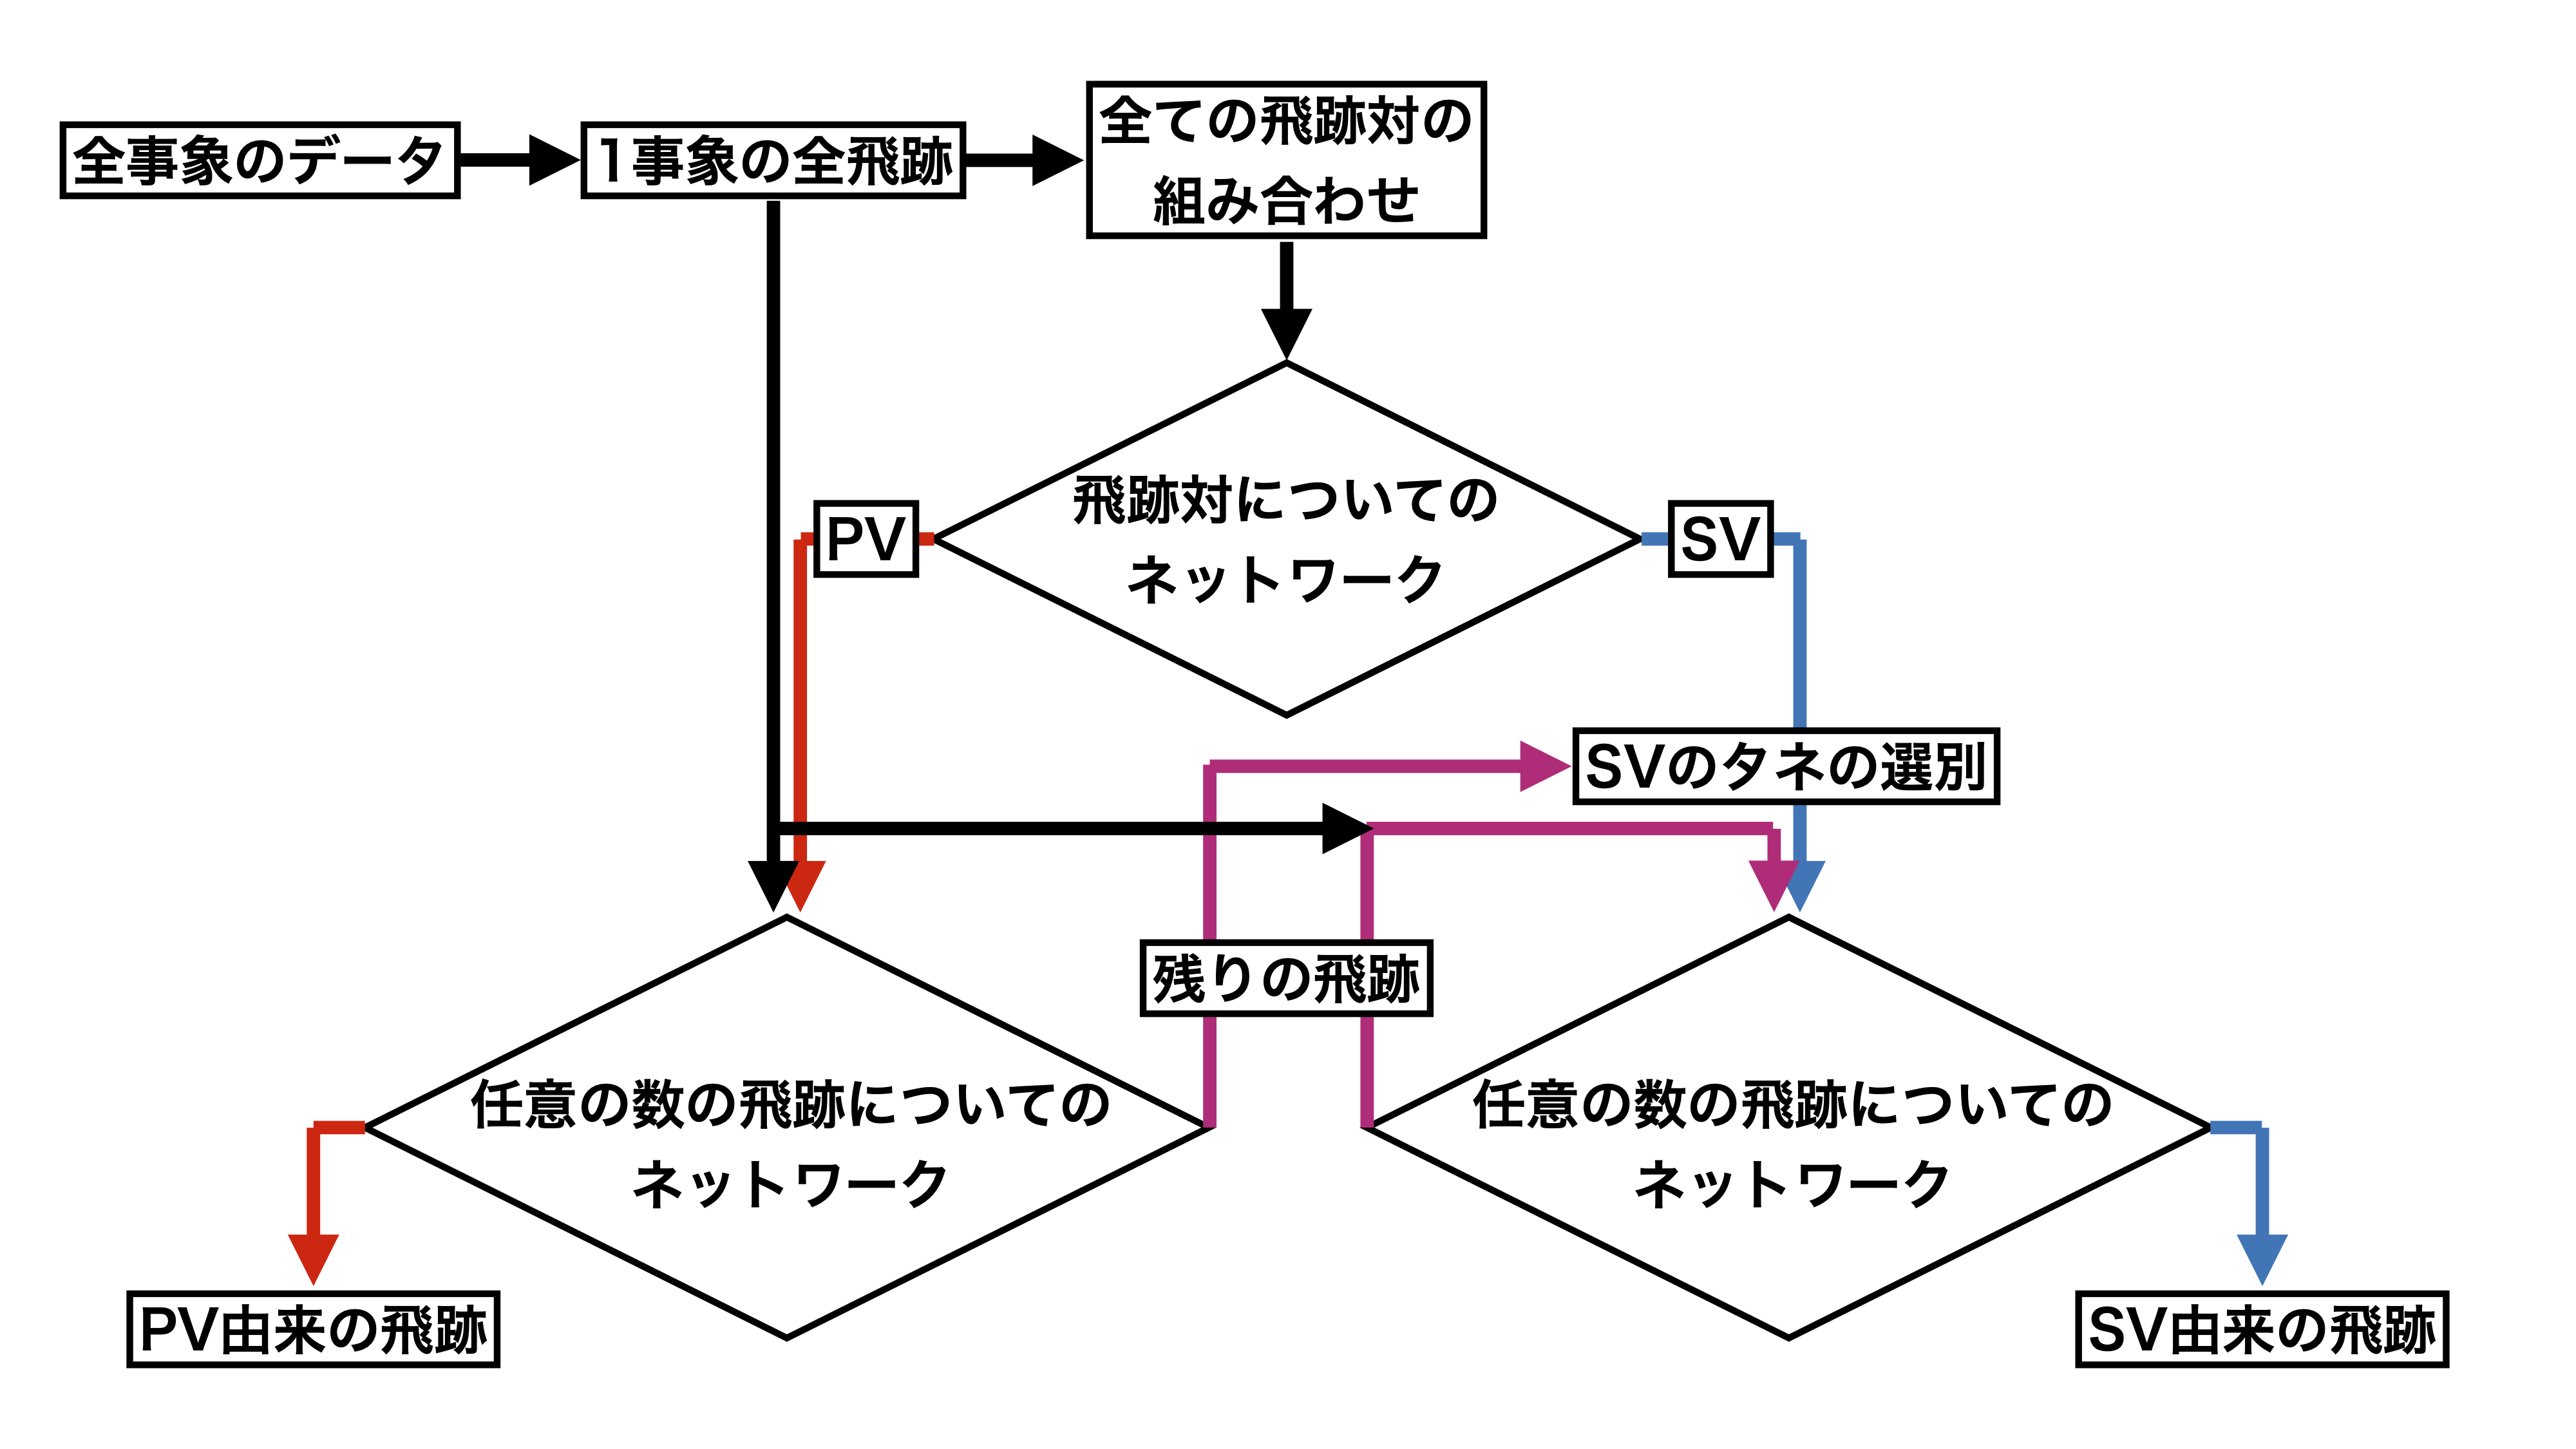
\includegraphics[width=0.9\textwidth, clip]{Figure/4VertexFinderwithDL/4-1-0-1VertexFinderAlgorithm.png}
 \caption{崩壊点検出アルゴリズム}
 \label{4-1-0-1VertexFinderAlgorithm}
\end{figure}

アルゴリズムは以下の手順で崩壊点の再構成を行う。

\begin{enumerate}
 \item 全事象から1事象分のデータを取り出し、全ての飛跡対の組み合わせを考える。
 \item それら飛跡対に対して、飛跡対についてのネットワークを使用し、崩壊点のタネの探索を行う。
 \item SVと判定された飛跡対について、選別を行いSVのタネを選ぶ。
 \item PVと判定されたタネについて、任意の数の飛跡についてのネットワークを用いPVの生成を行う。
 \item SVのタネとPV由来の飛跡の情報を用い、任意の数の飛跡についてのネットワークによってSVのタネが無くなるまでSVを生成する。
\end{enumerate}

手順1、2については飛跡対についてのネットワークの訓練データの作成や学習と全く同様の手順である。

手順3では、飛跡対についてのネットワークによって得られるSVCC・SVBB・TVCC・SVBCのスコアや崩壊点の位置を用いてより純度の高いSVのタネの集合を作成する。
したがって、SVCC・SVBB・TVCC・SVBCのスコアについての閾値や崩壊点の位置についての最適化が必要である。

手順4では、飛跡対についてのネットワークによって得られるPVのスコアについて降順に並び替えたPVのタネを用いて、個々に任意の数の飛跡についてのネットワークによってPVを生成する。
ここでは、PVのタネを幾つ用いるかについて最適化が必要である。
また一度以上、任意の数の飛跡についてのネットワークによって結合していると判定された飛跡をPV由来であると判断している。
この時の任意の数の飛跡についてのネットワークによって得られるスコアについての閾値についてもまた同様に最適化が必要なパラメータである。

手順5について、手順3で選別したSVのタネと手順4で得られたPV由来であると判定された飛跡の一覧を用いてSVの再構成を行う。
ここでは任意の数の飛跡についてのネットワークのデコーダー部に入力する飛跡から、再構成されたSV由来の飛跡を取り除いて行くことによって、再帰的にSVの生成が行われる。
SVのタネに含まれる飛跡はPV由来の飛跡の一覧になく、かつそれまでに生成したSV由来の飛跡の一覧にもないものを用いる。
このSVに関する任意の数の飛跡についてのネットワークのスコアも最適化が必要である。
また、再構成されたSV由来の飛跡の中にPV由来の飛跡が存在した場合は任意の数の飛跡についてのネットワークによって得られたスコアによって飛跡の争奪が行われる。
手順5はSVのタネが無くなるまで行われ、再構成されたSV由来の飛跡とPV由来の飛跡以外の飛跡は残りの飛跡とする。

以上が崩壊点検出のためのアルゴリズムである。
最適化が必要なパラメータを以下にまとめる。

\begin{itemize}
 \item 飛跡対についてのネットワークによって得られるSVCC・SVBB・TVCC・SVBCのスコアについての閾値
 \item 飛跡対についてのネットワークによって得られる崩壊点の位置についての閾値
 \item 使用するPVのタネの数
 \item PVの生成に関する任意の数の飛跡についてのネットワークによって得られるスコアについての閾値
 \item SVの生成に関する任意の数の飛跡についてのネットワークによって得られるスコアについての閾値
\end{itemize}


%%%%%%%%%%%%%%%%%%%%%%%%%%%%%%%%%%%%%%%%%%%%%%%%%%%%%%%%%%%%%%%%%%%%%%%%%%%%%%%%%%%%%%%%%%%%%%%%%%%%%
\section{崩壊点検出の最適化と評価} \label{VFDL:TuneandPerformanceofVFDL}

崩壊点検出の最適化では、まず、飛跡対についてのネットワークによって得られるSVCC・SVBB・TVCC・SVBCのスコアについての閾値と崩壊点の位置についての閾値の最適化を行う。
次に、使用するPVのタネの数、PV、SVの生成に関する任意の数の飛跡についてのネットワークによって得られるスコアについての閾値の最適化を行う。
前者はSVのタネの探索に関するパラメータ、後者は崩壊点の生成や全体性能についてのパラメータである。


%%%%%%%%%%%%%%%%%%%%%%%%%%%%%%%%%%%%%%%%%%%%%%%%%%%%%%%%%%%%%%%%%%%%%%%%%%%%%%%%%%%%%%%%%%%%%%%%%%%%%
\subsection{SVのタネの探索} \label{VFDL:TPVFDL:SVSeedSelection}

SVのタネを探索する上での評価基準は純度と効率である。
ここでは、SVのタネの効率や純度について、SVCC・SVBB・TVCC・SVBCのスコアの和に対する閾値と崩壊点の位置についての閾値を変化させ最適な値を探る。
ただし、崩壊点検出アルゴリズムではここから更にPV由来である飛跡を含むタネを除外する為、その純度は改善されると考えられる。
また、SVのタネの選別におけるPre-Selectionとして、飛跡対についてのネットワークでNC・PV・Othersと判定された飛跡対を取り除いている。
以上より、SVのタネについての効率と純度を次のように定義する
\begin{equation}
 \begin{split}
{\rm Efficiency = \frac{less\ than\ Vertex\ Position\ and\ more\ than\ Score\ and\ True\ SV\ Seed}{True\ SV\ Seed}}\\
{\rm Purity = \frac{less\ than\ Vertex\ Position\ and\ more\ than\ Score\ and\ True\ SV\ Seed}{less\ than\ Vertex\ Position\ and\ more\ than\ Score}}
 \end{split}
\end{equation}
閾値とSVのタネの効率、純度の関係を図\ref{4-2-1-1SVSeed}に示す。

\begin{figure}[htbp]
 \centering
 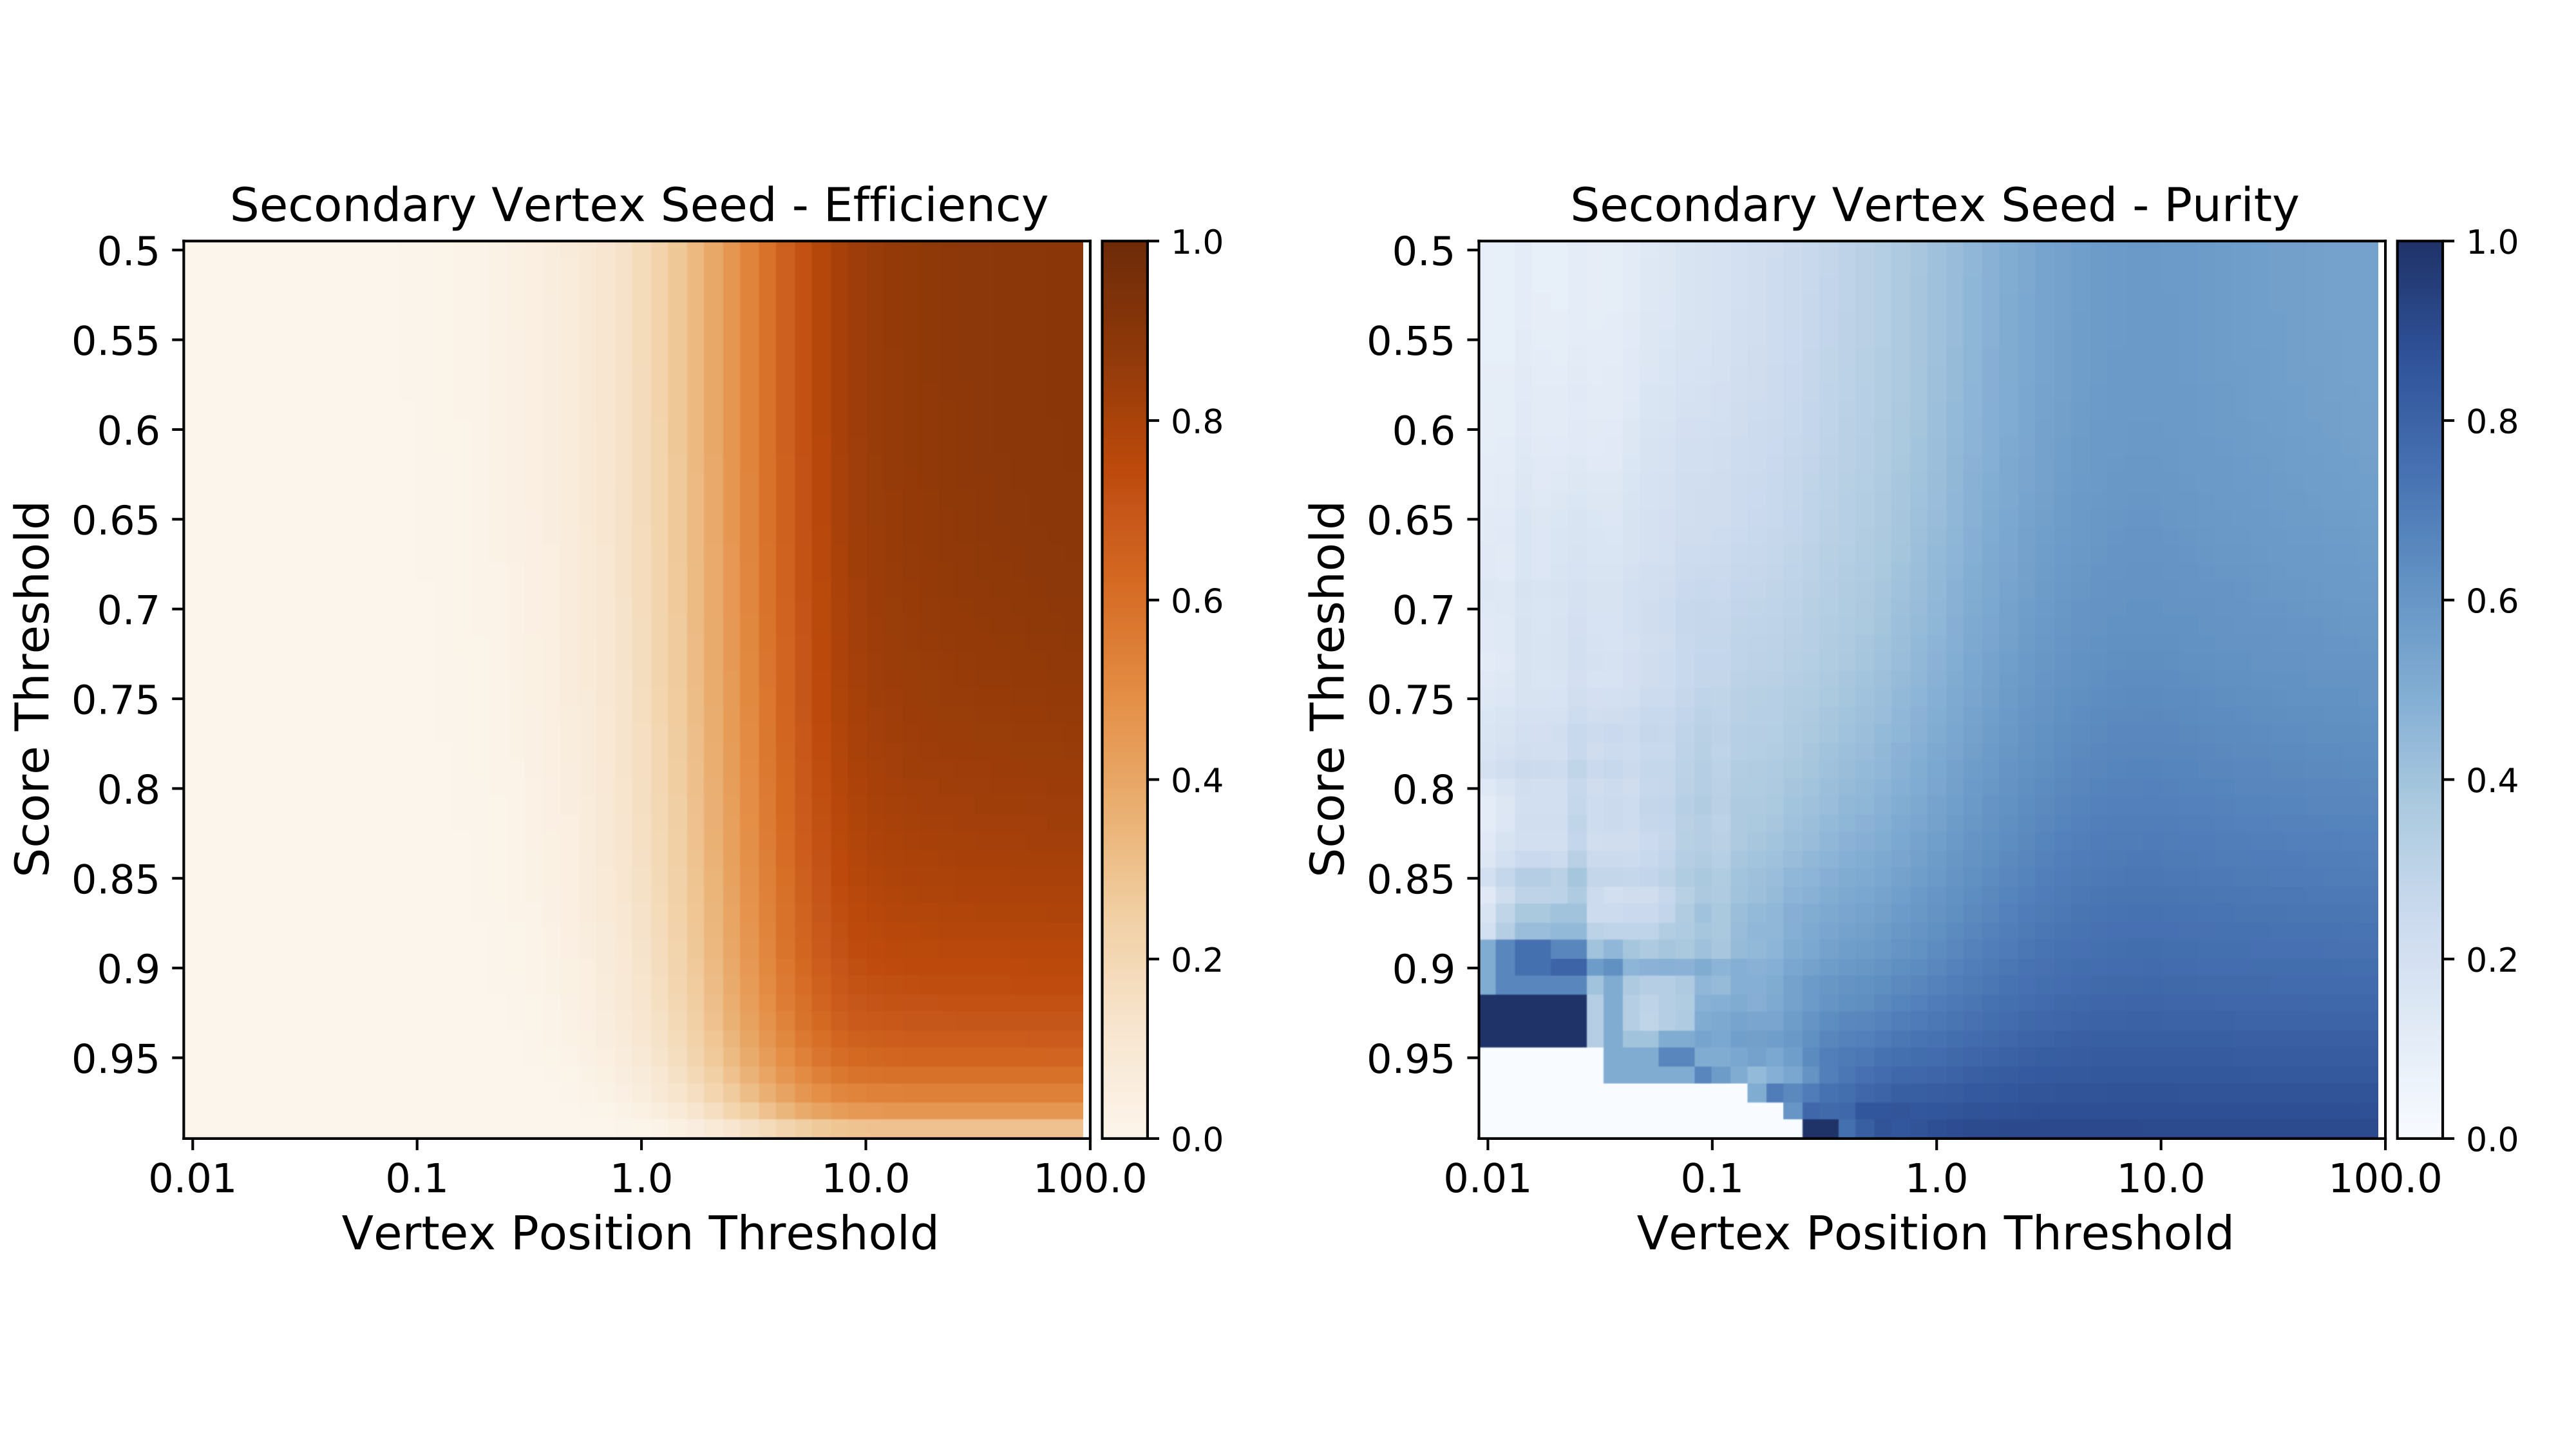
\includegraphics[width=0.9\textwidth, clip]{Figure/4VertexFinderwithDL/4-2-1-1SVSeed.png}
 \caption[閾値とSVのタネの効率、純度の関係]{閾値とSVのタネの効率、純度の関係。図左が効率についての関係、図右が純度についての関係である。縦軸はSVについてのスコアの和に対しての閾値、横軸は崩壊点の位置についての閾値を示している。また、横軸についてはログスケールを用いている。}
 \label{4-2-1-1SVSeed}
\end{figure}

効率については、SVの位置がビーム衝突点から$1$から$10\ \mathrm{mm}$でピークを持つことからも分かるように崩壊点の位置についての閾値をより大きくすることによって改善されている。
一方、スコアについての閾値は位置と比較して変化が小さく、$0.8$程度から徐々に効率が減少している。
このことから、SVCC・SVBB・TVCC・SVBCのスコアの和は比較的大きな値を持っていることが理解できる。
純度については、崩壊点の位置についての閾値が小さく、かつスコアについての閾値が大きな領域においては選択されたSVのタネが存在しなかった為、$0$としている。
また、全体の傾向として、崩壊点の位置についての閾値が一定で、スコアについての閾値が大きい領域で純度が高くなっている。
これは、前述したような崩壊点の位置の特性や深層学習のスコアから明らかな性質である。

最適なパラメータの設定のため、Precision-Recall (PR) 曲線を使用する (図\ref{4-2-1-2PRCurve})。
ここで、Precisionは純度、Recallは効率である。
図\ref{4-2-1-1SVSeed}からも明らかな様に効率は崩壊点の位置についての閾値が$1\ \mathrm{mm}$の辺りで急速に減少している。
したがって、崩壊点の位置についての閾値が$1\ \mathrm{mm}$以上の場合についてのみ考えることとする。
また、性能の最大値として効率と純度の和が最大となるパラメータの組み合わせを用いる。。
このパラメータは以降の崩壊点の生成や崩壊点検出の性能、現行の手法との比較に用いる。

\begin{figure}[htbp]
 \centering
 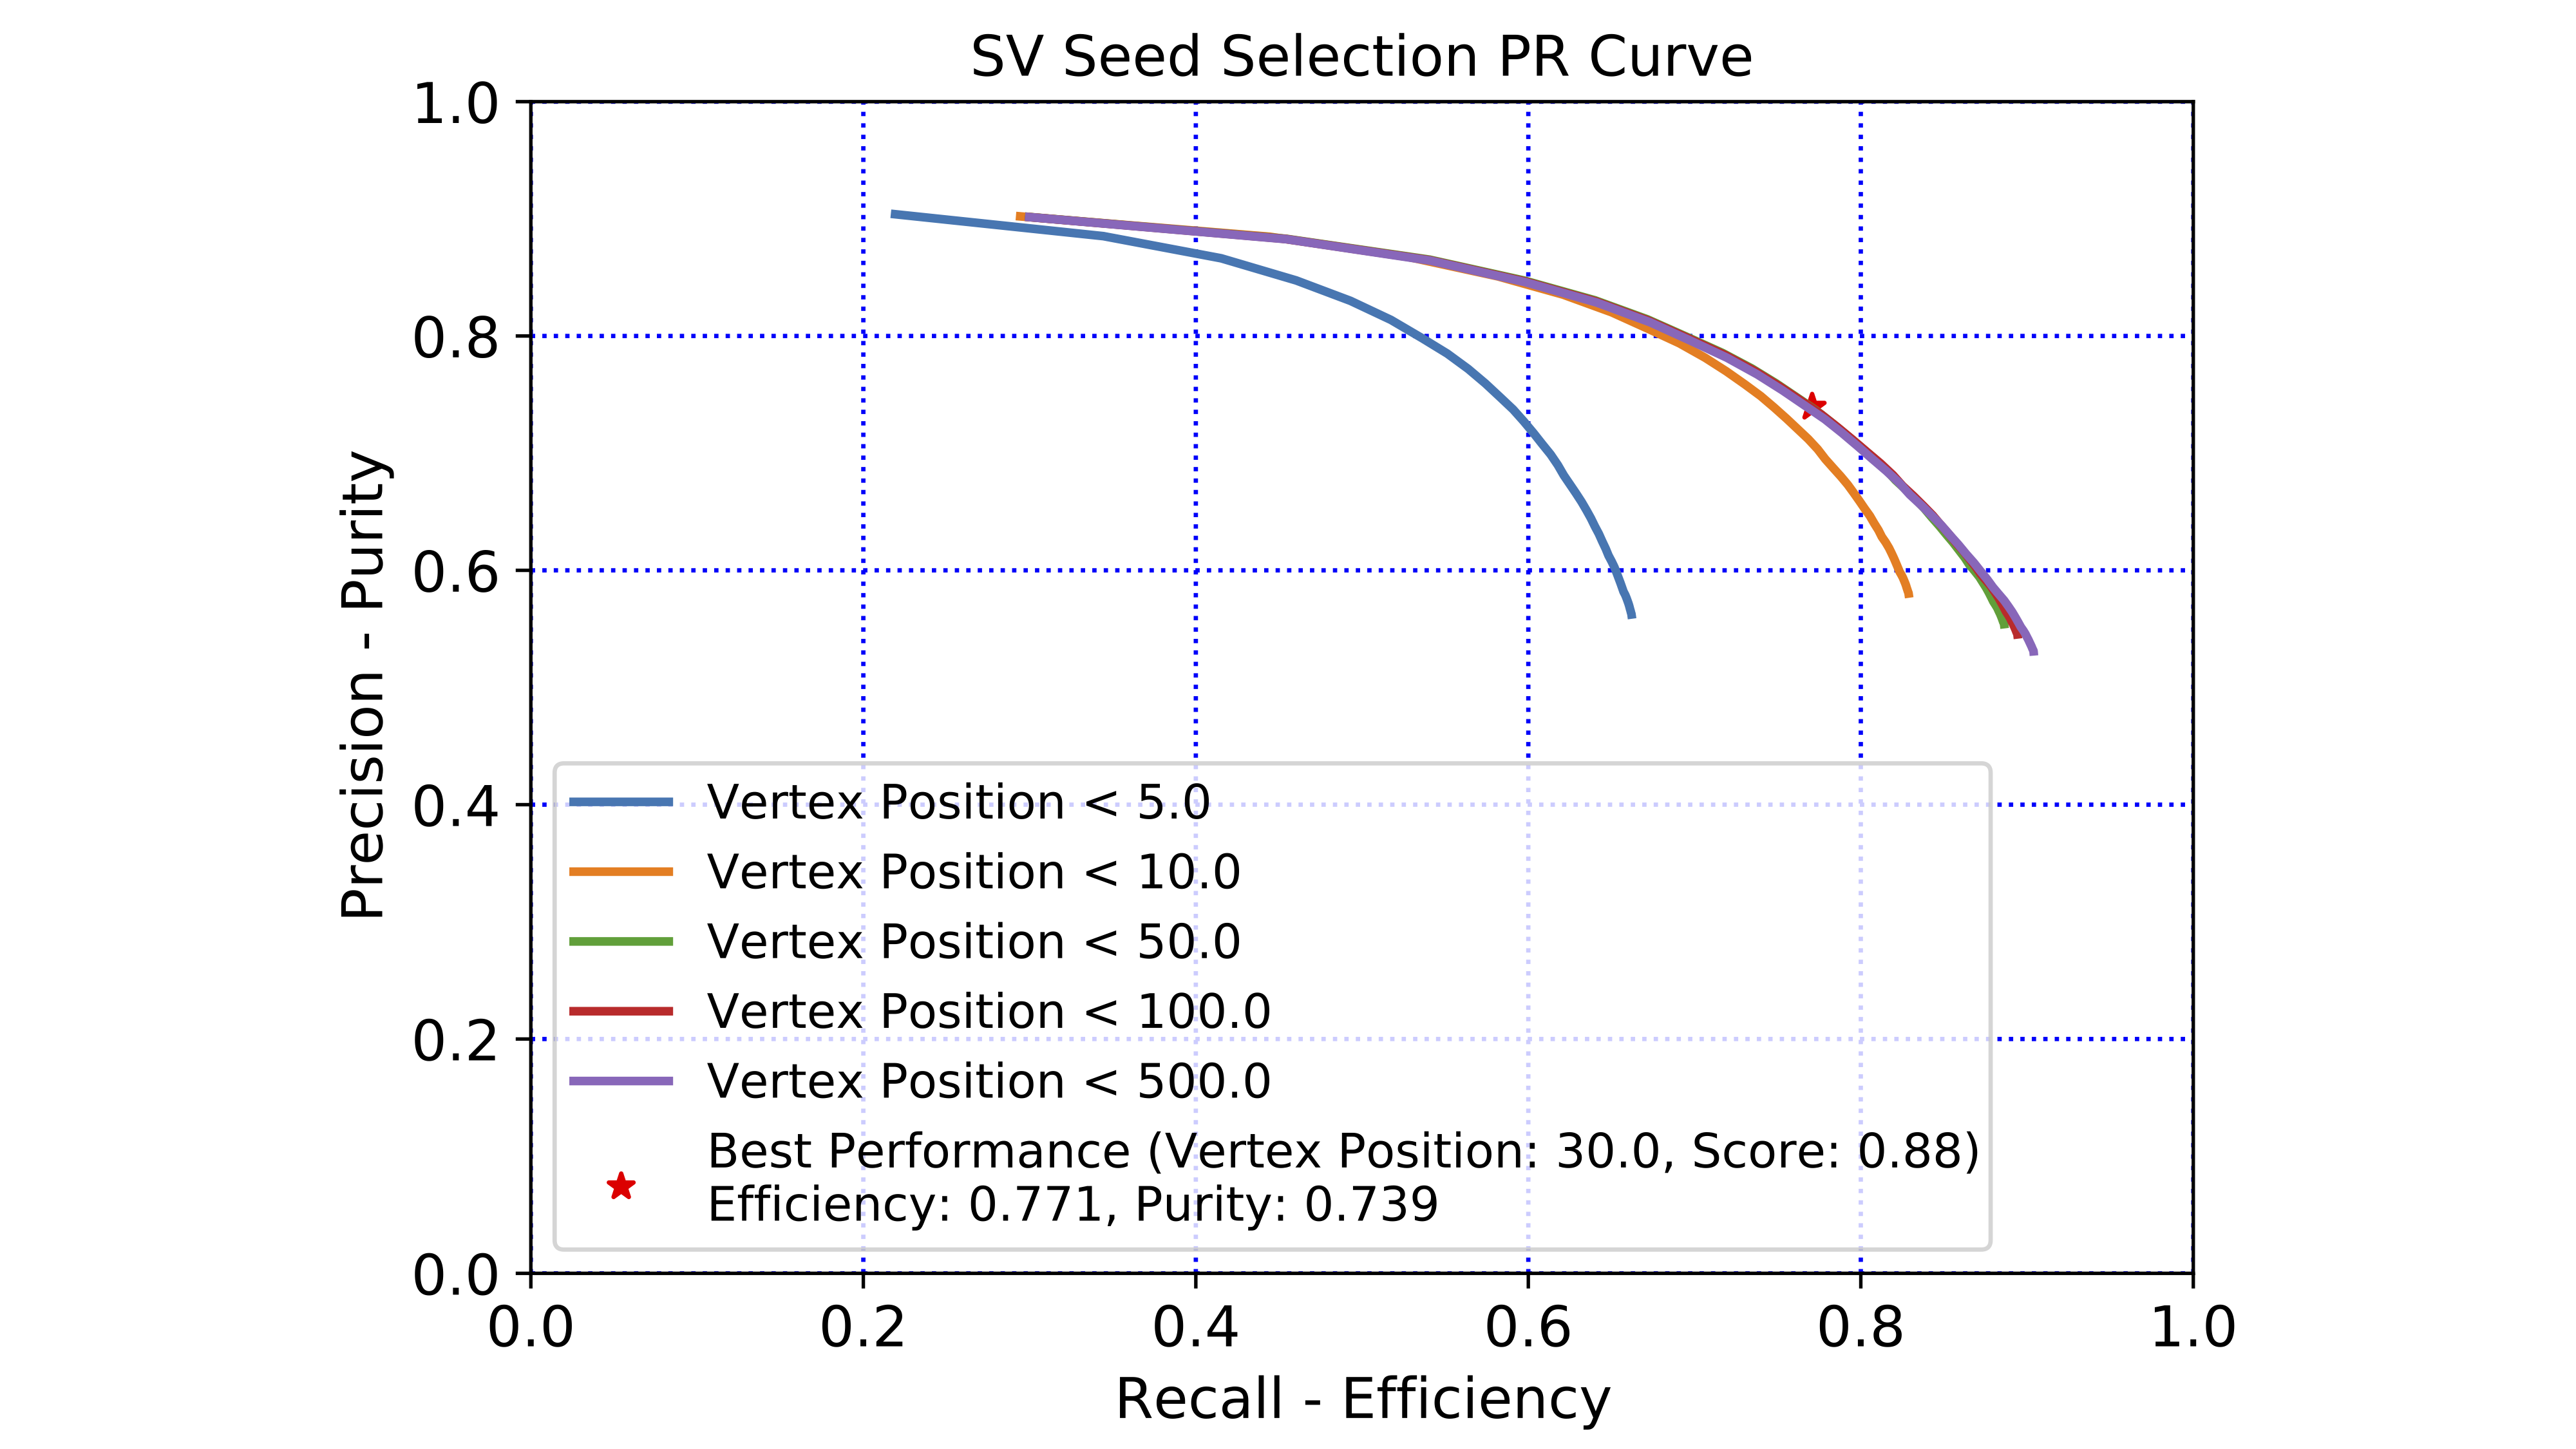
\includegraphics[width=0.9\textwidth, clip]{Figure/4VertexFinderwithDL/4-2-1-2PRCurve.png}
 \caption[閾値とSVのタネの効率、純度についてのPR曲線]{閾値とSVのタネの効率、純度についてのPR曲線。縦軸は純度、横軸は効率である。崩壊点の位置についての閾値を固定し、スコアについての閾値を変化させている。崩壊点の位置については$5.0,\ 10.0,\ 50.0,\ 100.0,\ 500.0\ {\mathrm mm}$のデータのみ描画している。}
 \label{4-2-1-2PRCurve}
\end{figure}

図\ref{4-2-1-2PRCurve}では、崩壊点の位置については$5.0,\ 10.0,\ 50.0,\ 100.0,\ 500.0\ {\mathrm mm}$のデータのみ描画しているが、実際には$1.0-9.0$まで$1$刻みずつ、$10.0-90.0$まで$10$刻みずつ$100-900$まで$100$刻みずつのデータについて最適なパラメータの探索を行った。
また、スコアについては$0.50-0.99$まで$0.01$刻みでの探索を行った。


%%%%%%%%%%%%%%%%%%%%%%%%%%%%%%%%%%%%%%%%%%%%%%%%%%%%%%%%%%%%%%%%%%%%%%%%%%%%%%%%%%%%%%%%%%%%%%%%%%%%%
\subsection{崩壊点の生成} \label{VFDL:TPVFDL:VertexProduction}

崩壊点の生成や全体性能についてのパラメータを最適化する為、崩壊点検出の性能の評価項目を定める必要がある。
そのような評価項目は飛跡についての効率を用いている。
詳細を以下に示す。

\begin{itemize}
 \item MCPrimaryRecoSV : MC情報によってPV由来の飛跡であるとラベルされた飛跡の内、ネットワークがどの程度SVと判断してしまったか
 \item MCOthersRecoSV : MC情報によってOthersであるとラベルされた飛跡の内、ネットワークがどの程度SVと判断してしまったか
 \item MCBottomRecoSV : MC情報によってボトム・フレーバーのSV由来であるとラベルされた飛跡の内、ネットワークがどの程度SVと判断できたか
 \item MCCharmRecoSV : MC情報によってチャーム・フレーバーのSV由来であるとラベルされた飛跡の内、ネットワークがどの程度SVと判断できたか
\end{itemize}

MCPrimaryRecoSVやMCOthersRecoSVは値が小さければ小さいほど性能が高く、それ以外の評価項目は値が大きいほど性能が高いと判断する。
更に、ボトム・フレーバー、チャーム・フレーバーのSV由来である飛跡については以下の評価を行う。

\begin{itemize}
 \item SameChain : 同一の崩壊チェイン由来の飛跡のみで構成されているか
 \item SameParticle : 同一の親粒子由来の飛跡のみで構成されているか
\end{itemize}

ここでは、ボトム・フレーバー、チャーム・フレーバーのSVの内、同じボトム・ハドロンから生じたSVの組みを崩壊チェインと呼び、更に細かく個々のSVを親粒子と呼んでいる (図\ref{4-2-2-1SameChainSameParticle})。
同一の崩壊チェイン、同一の親粒子とはこれらの崩壊チェインや親粒子を跨いで飛跡を選択しているかどうかを判断している。

\begin{figure}[htbp]
 \centering
 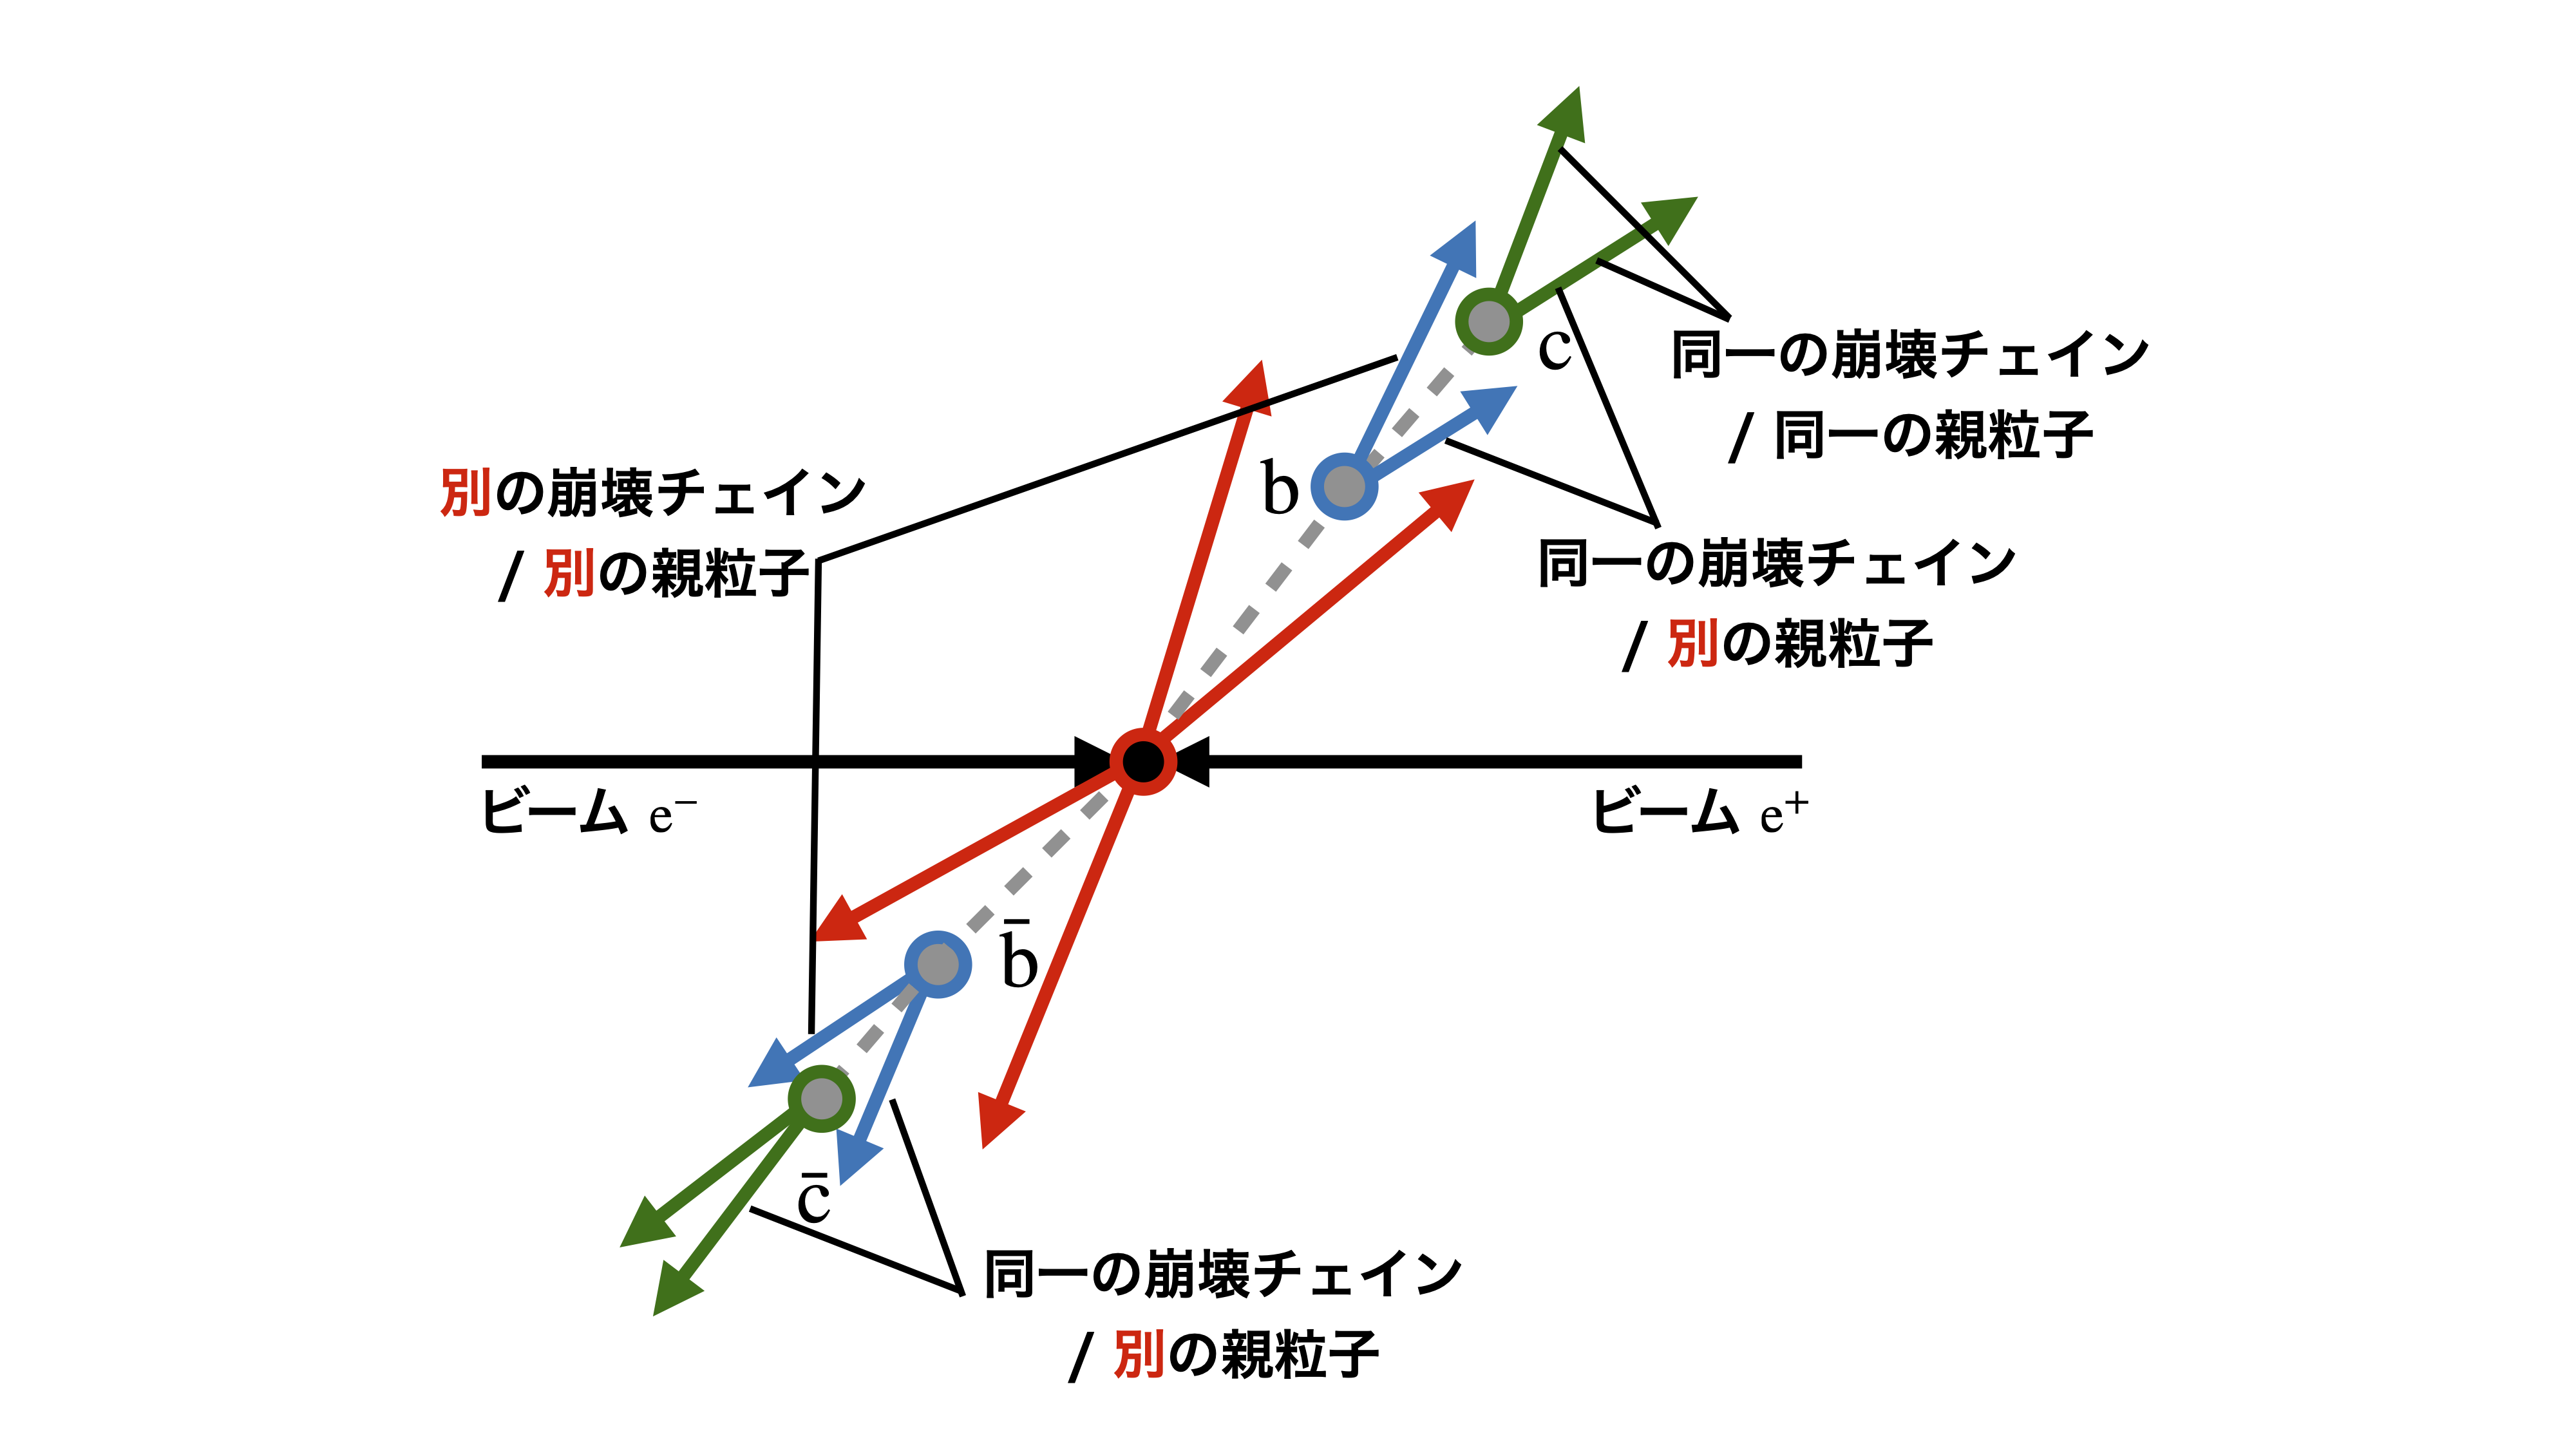
\includegraphics[width=0.9\textwidth, clip]{Figure/4VertexFinderwithDL/4-2-2-1SameChainSameParticle.png}
 \caption[同一の崩壊チェインと同一の親粒子]{同一の崩壊チェインと同一の親粒子}
 \label{4-2-2-1SameChainSameParticle}
\end{figure}

これらの評価項目は前述した現行の手法であるLCFIPlusでの評価項目と同じものである。
また、同一の崩壊チェインなどの基準は終状態$\rm b\bar{b}$でしか起こり得ないことについても注意が必要である。
したがってこれらの評価は基本的には終状態$\rm b\bar{b}$のデータを用いて行うこととなる。

崩壊点の生成や全体性能についてのパラメータは使用するPVのタネの数、PV、SVの生成におけるネットワークのスコアの閾値の三つである。
それぞれ三つのパラメータについて、PVのタネの数を$1$から$3$個まで、PV、SVのスコアの閾値を$0.5$から$0.95$まで変化させ、各評価項目の値を確認する。
結果を図\ref{4-2-2-2TrackEfficiency},\ref{4-2-2-3TrackEfficiency},\ref{4-2-2-4TrackEfficiency}に示す。

\begin{figure}[htbp]
 \centering
  %\begin{tabular}{cccc}
  \begin{minipage}{1.0\textwidth}
   \centering
    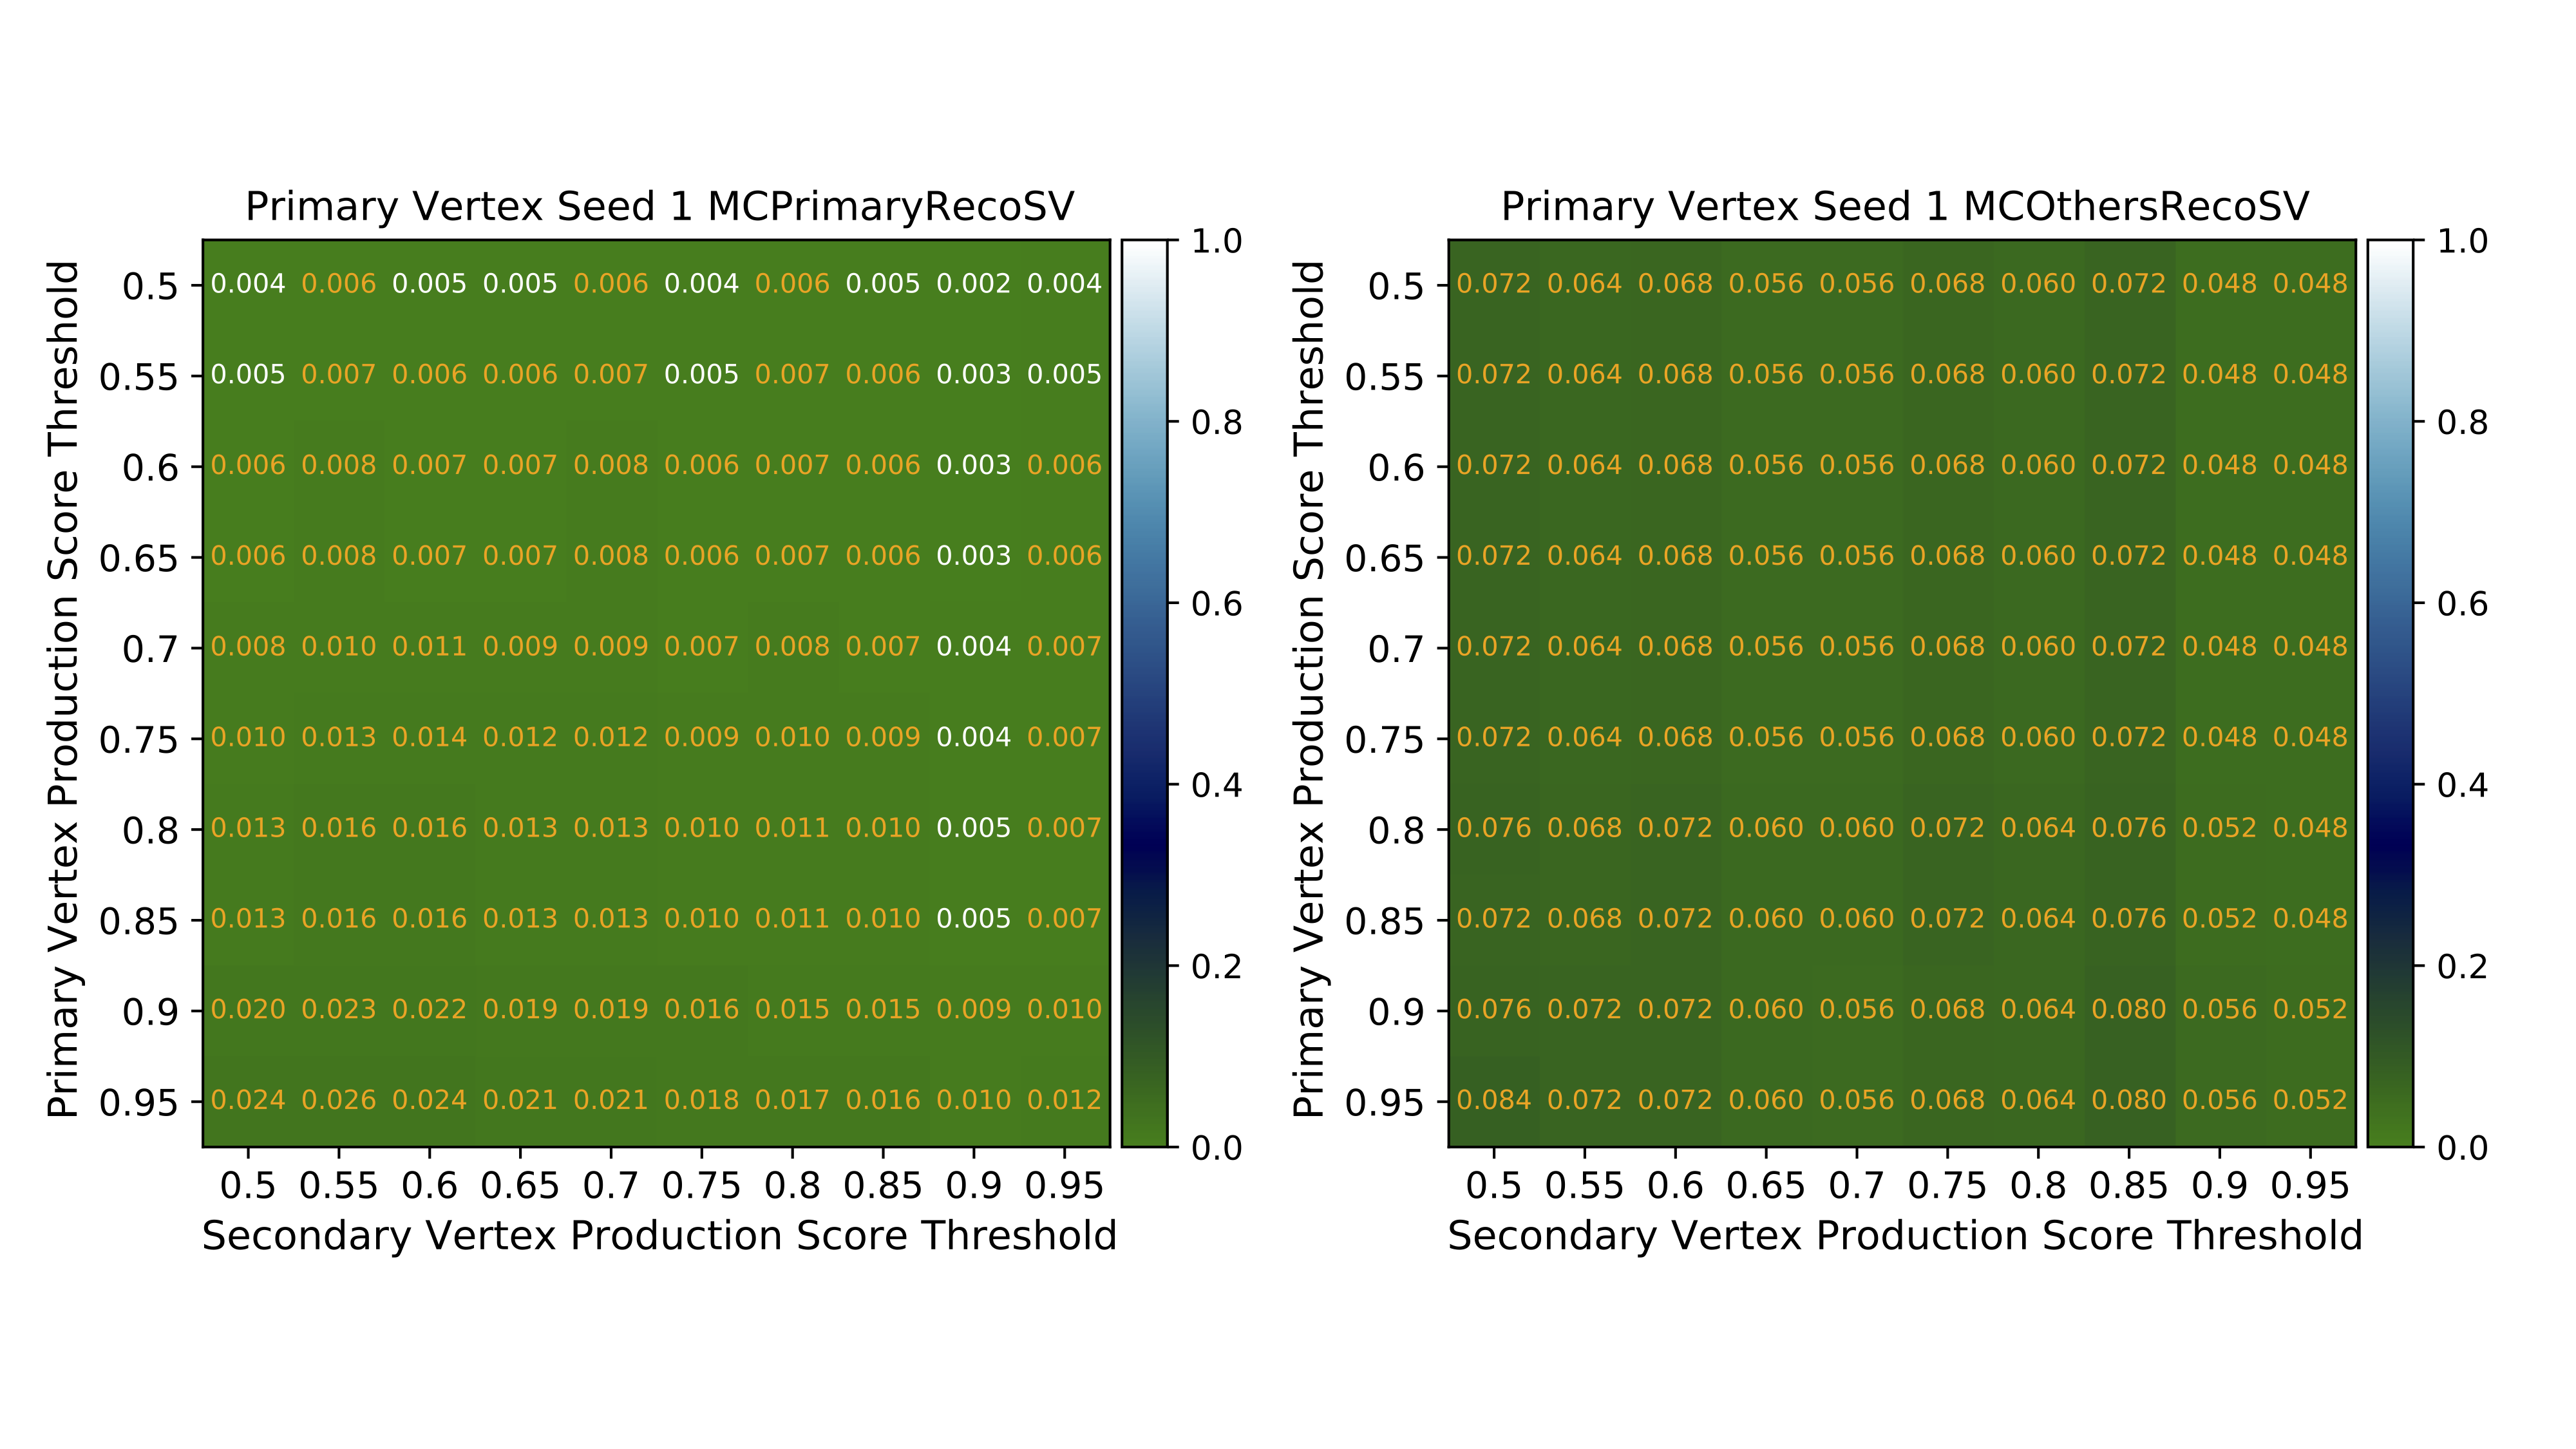
\includegraphics[trim = 0 140 0 140, width=0.95\textwidth, clip]{Figure/4VertexFinderwithDL/4-2-2-2TrackEfficiencyPVOthers.png}
   \end{minipage}
   
   \begin{minipage}{1.0\textwidth}
   \centering
    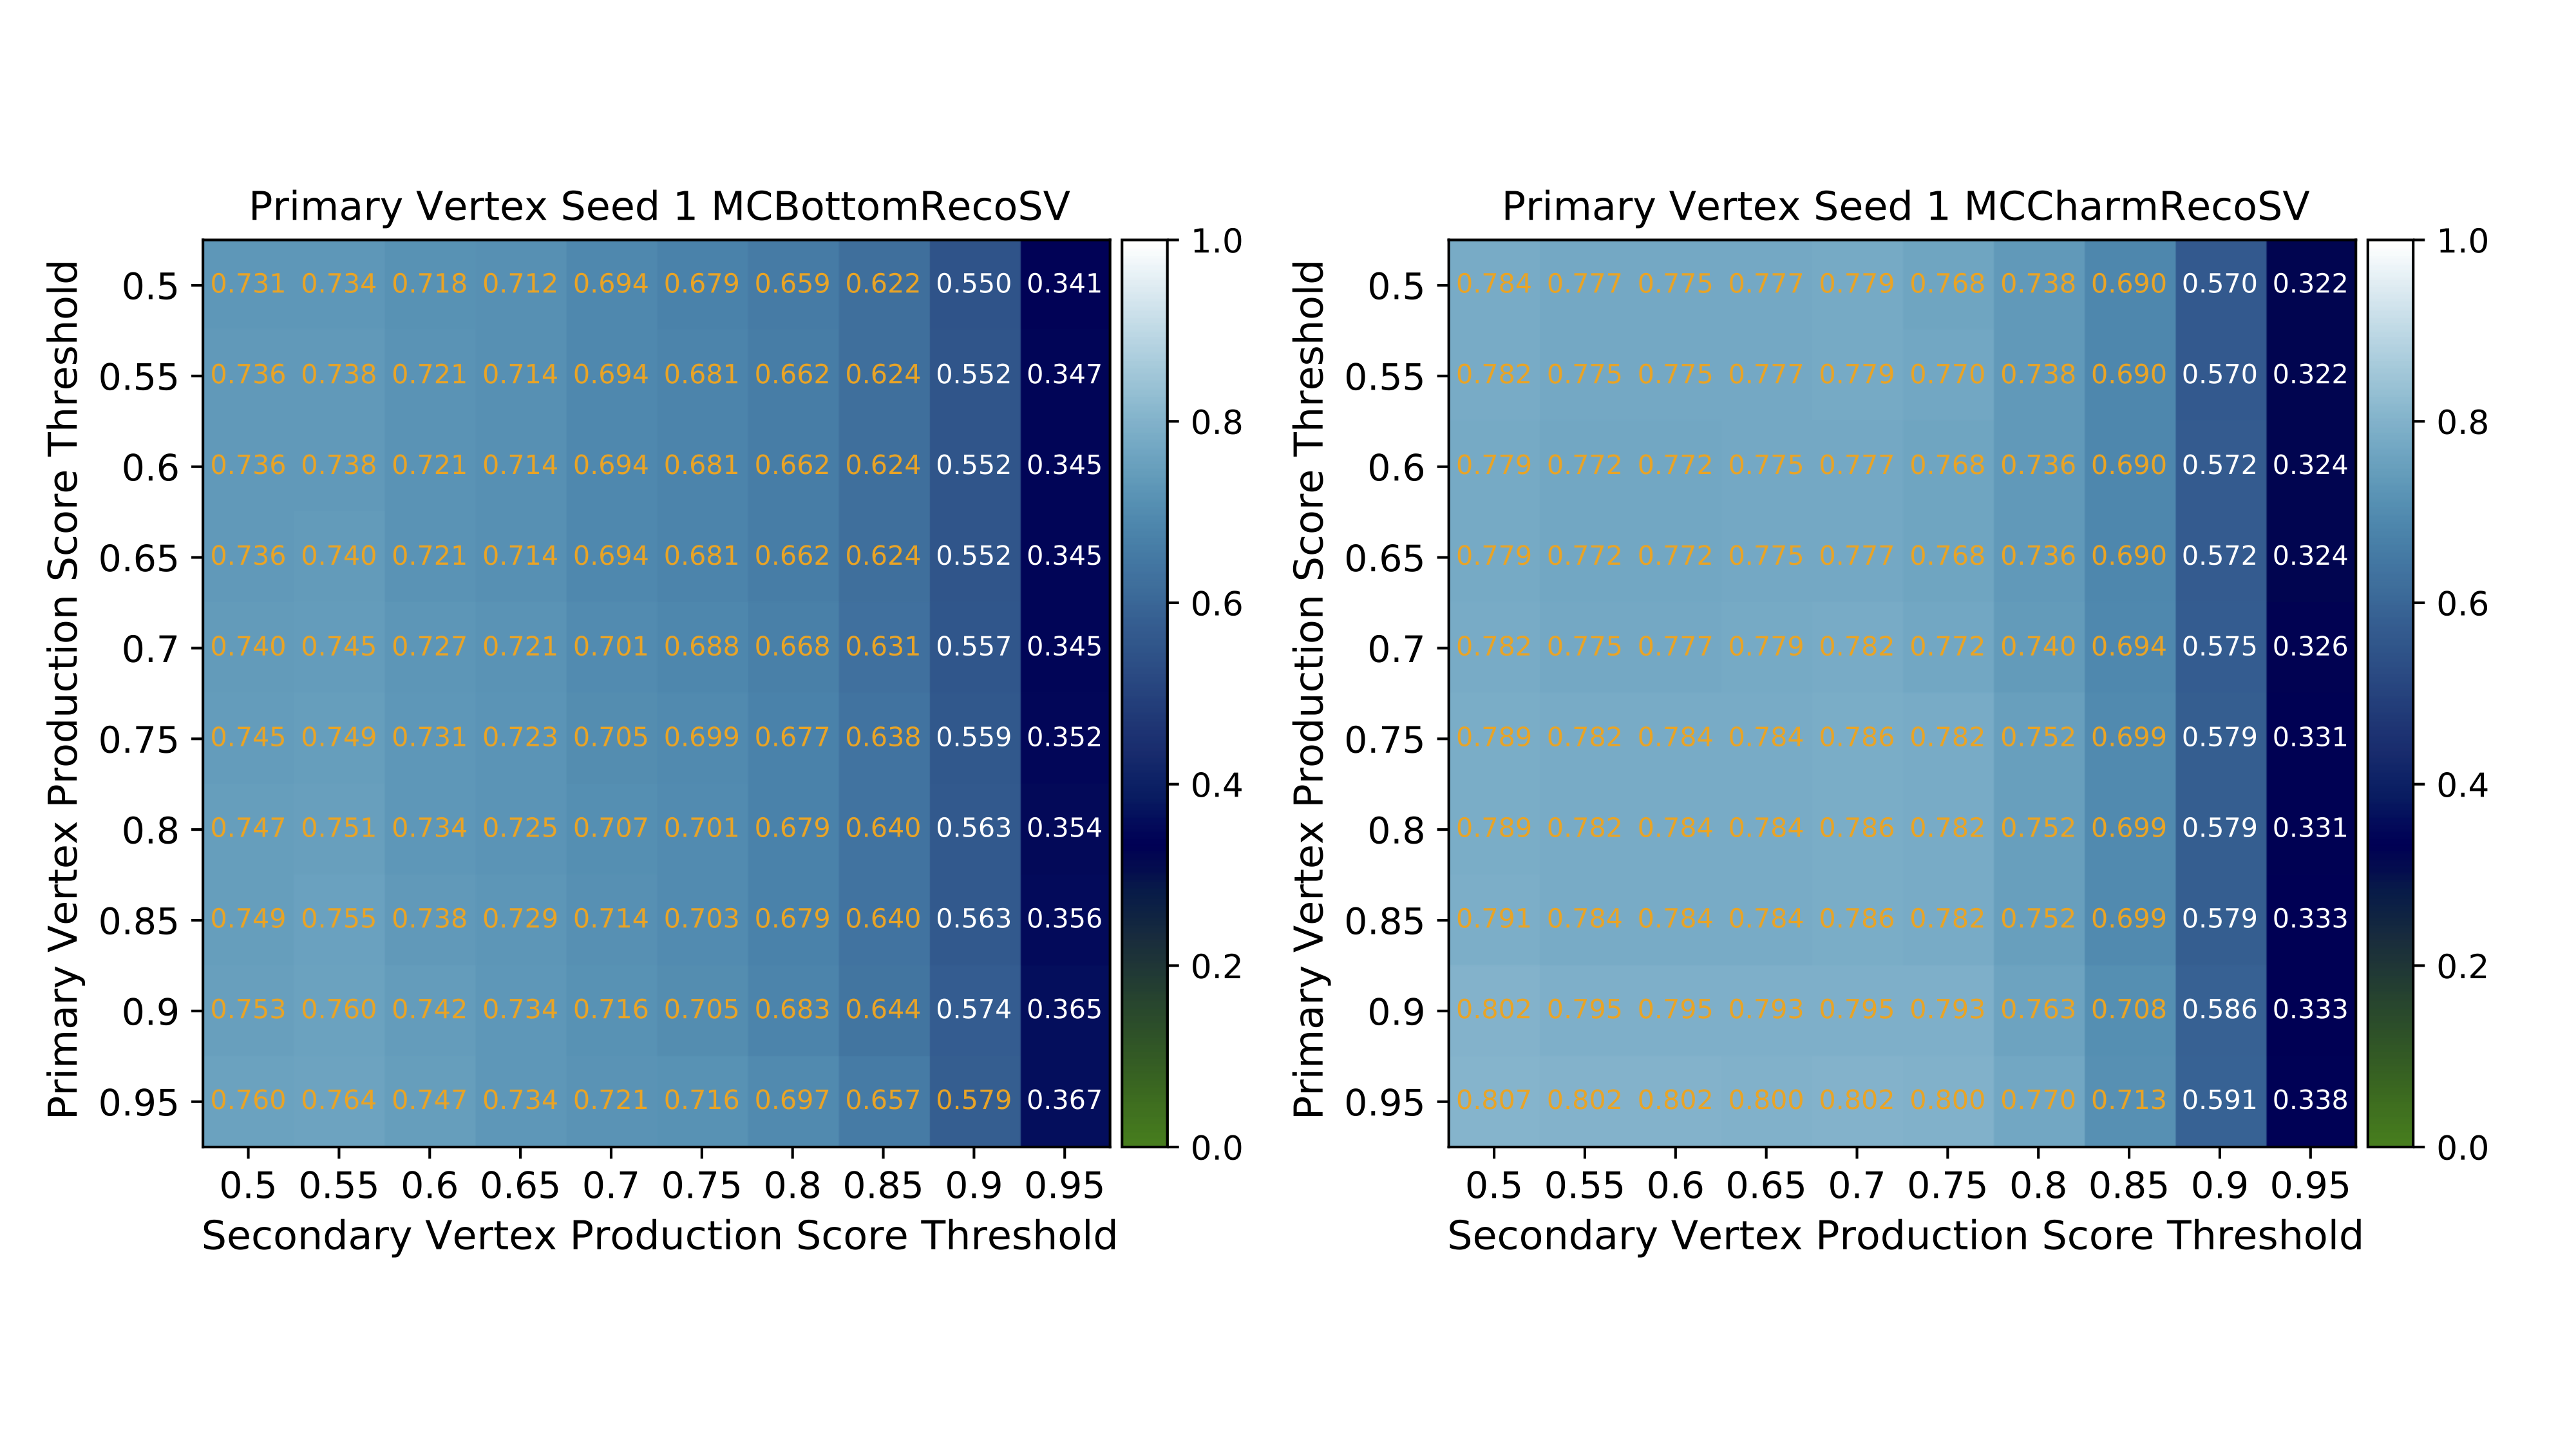
\includegraphics[trim = 0 140 0 140, width=0.95\textwidth, clip]{Figure/4VertexFinderwithDL/4-2-2-2TrackEfficiencyBottomCharm.png}
   \end{minipage}
   
   \begin{minipage}{1.0\textwidth}
   \centering
    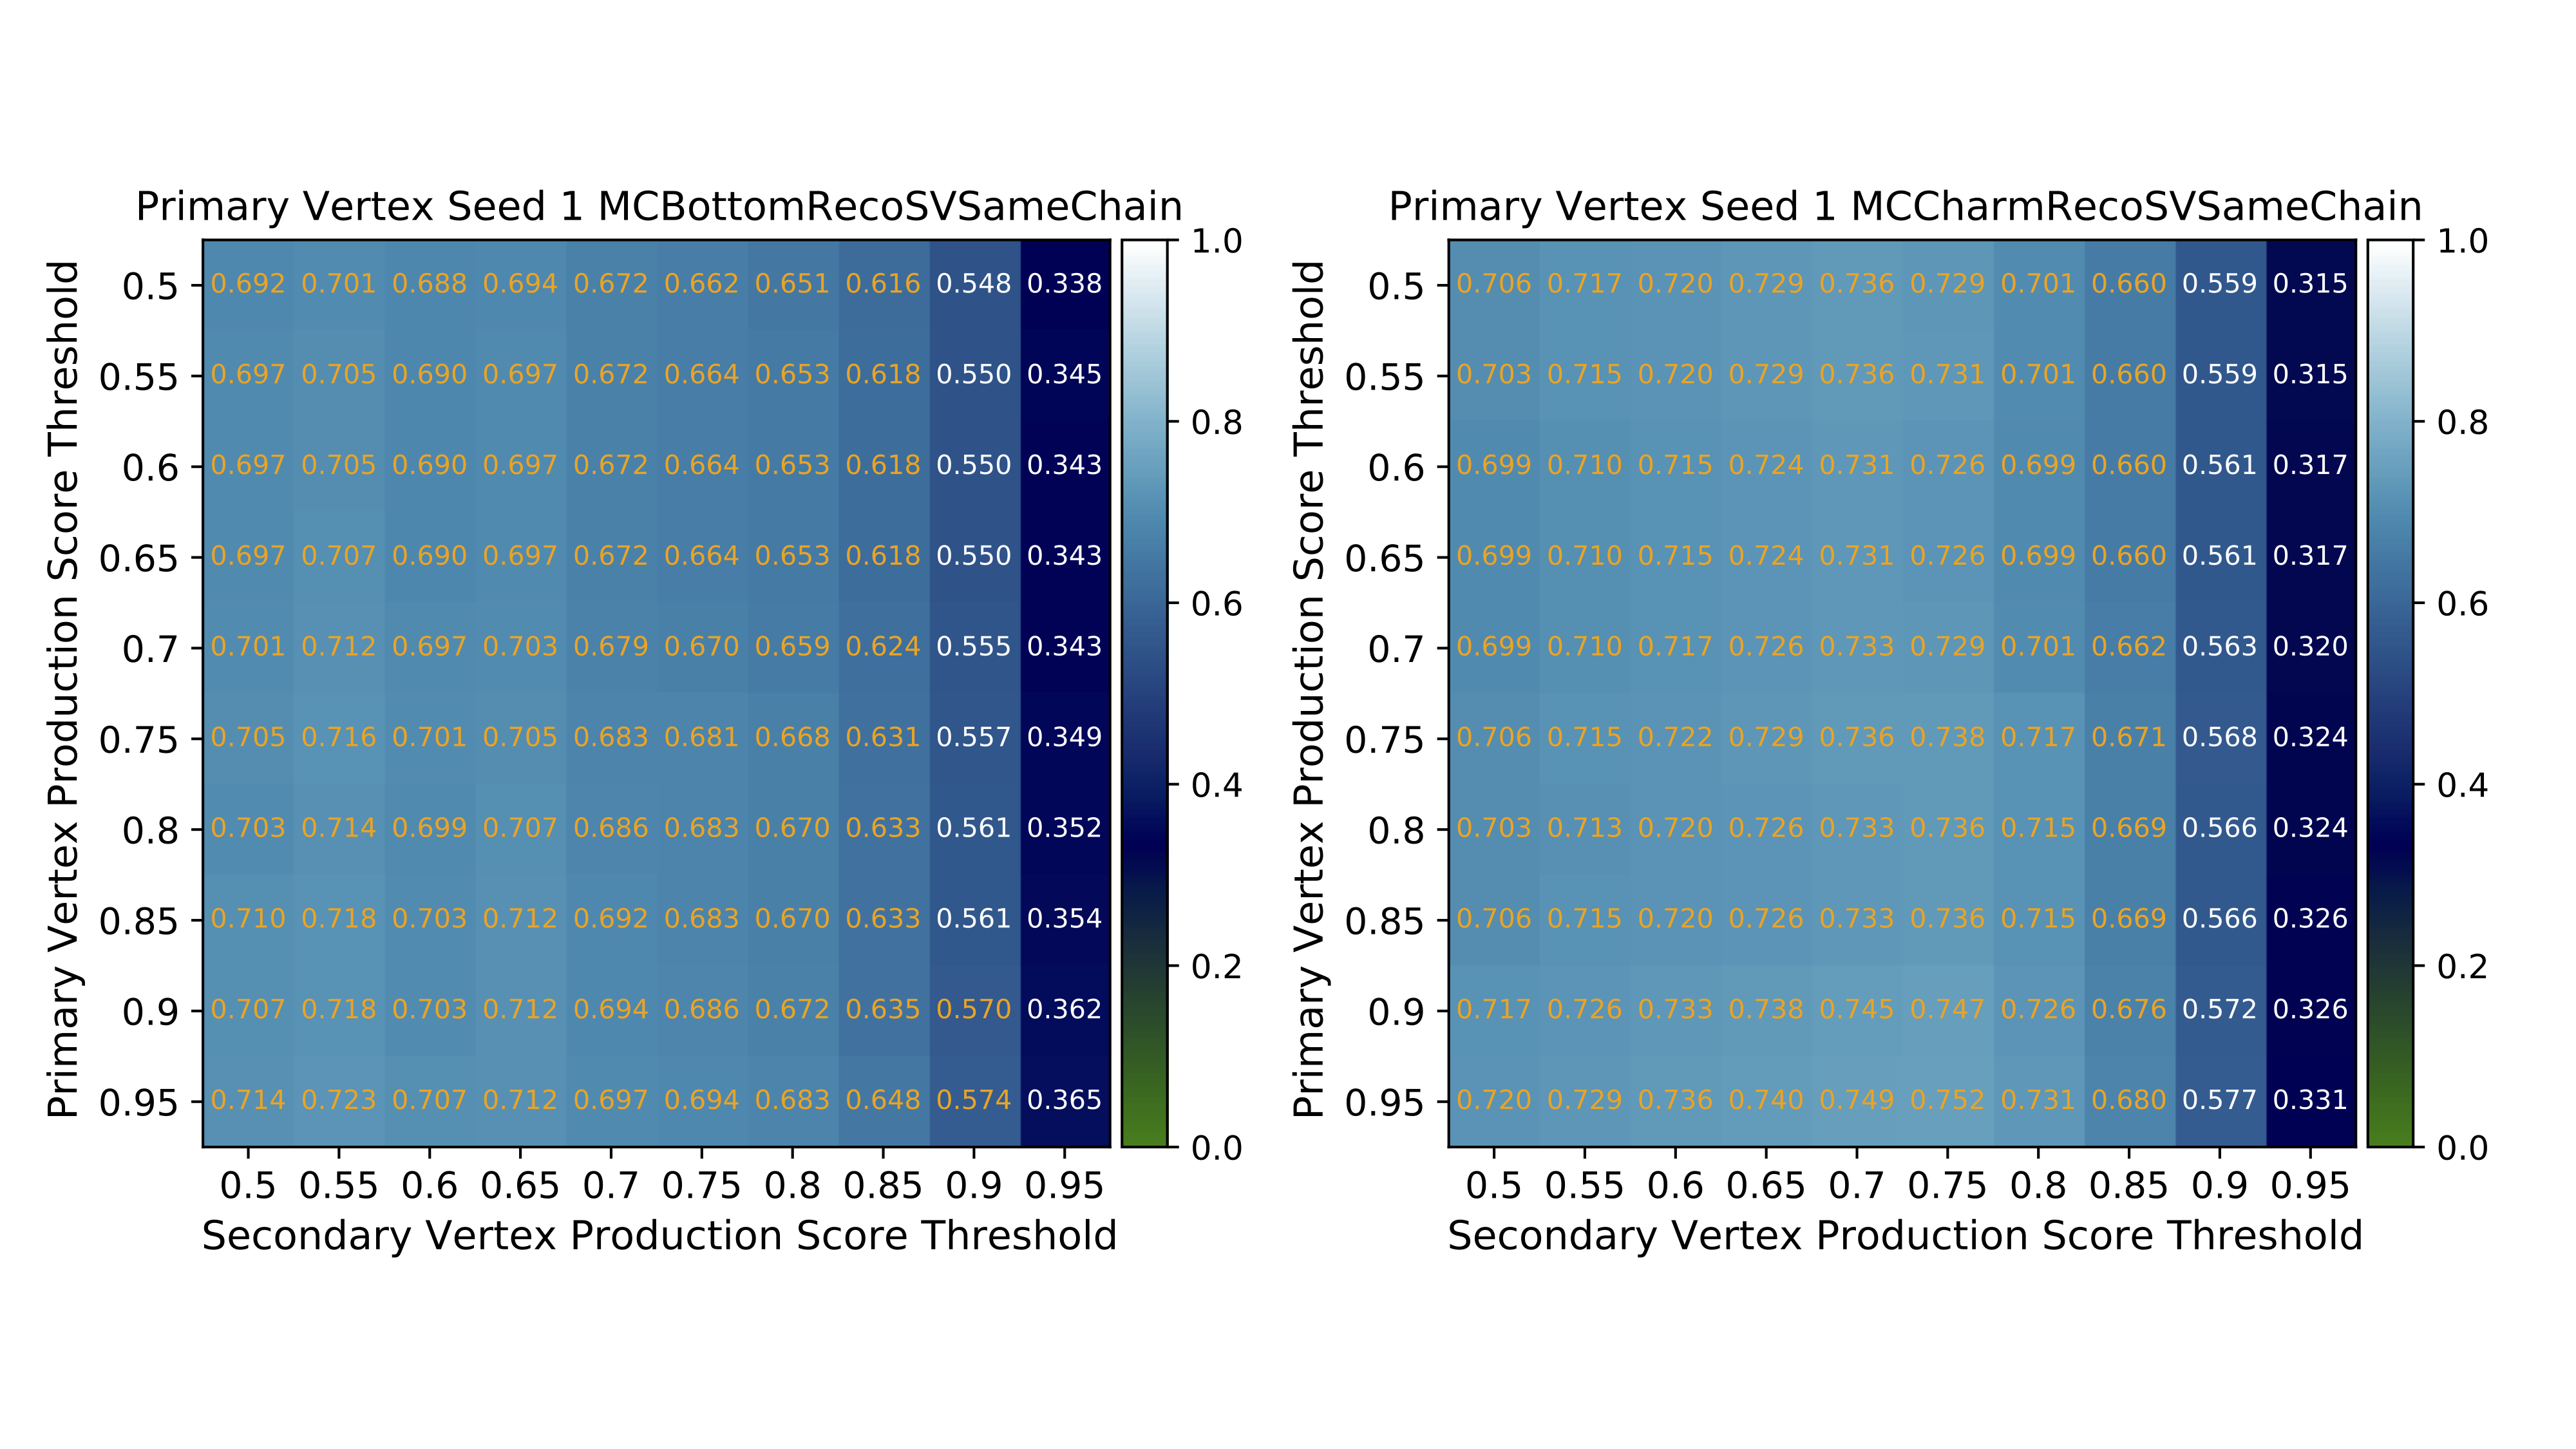
\includegraphics[trim = 0 140 0 140, width=0.95\textwidth, clip]{Figure/4VertexFinderwithDL/4-2-2-2TrackEfficiencySameChain.png}
   \end{minipage}
   
   \begin{minipage}{1.0\textwidth}
   \centering
    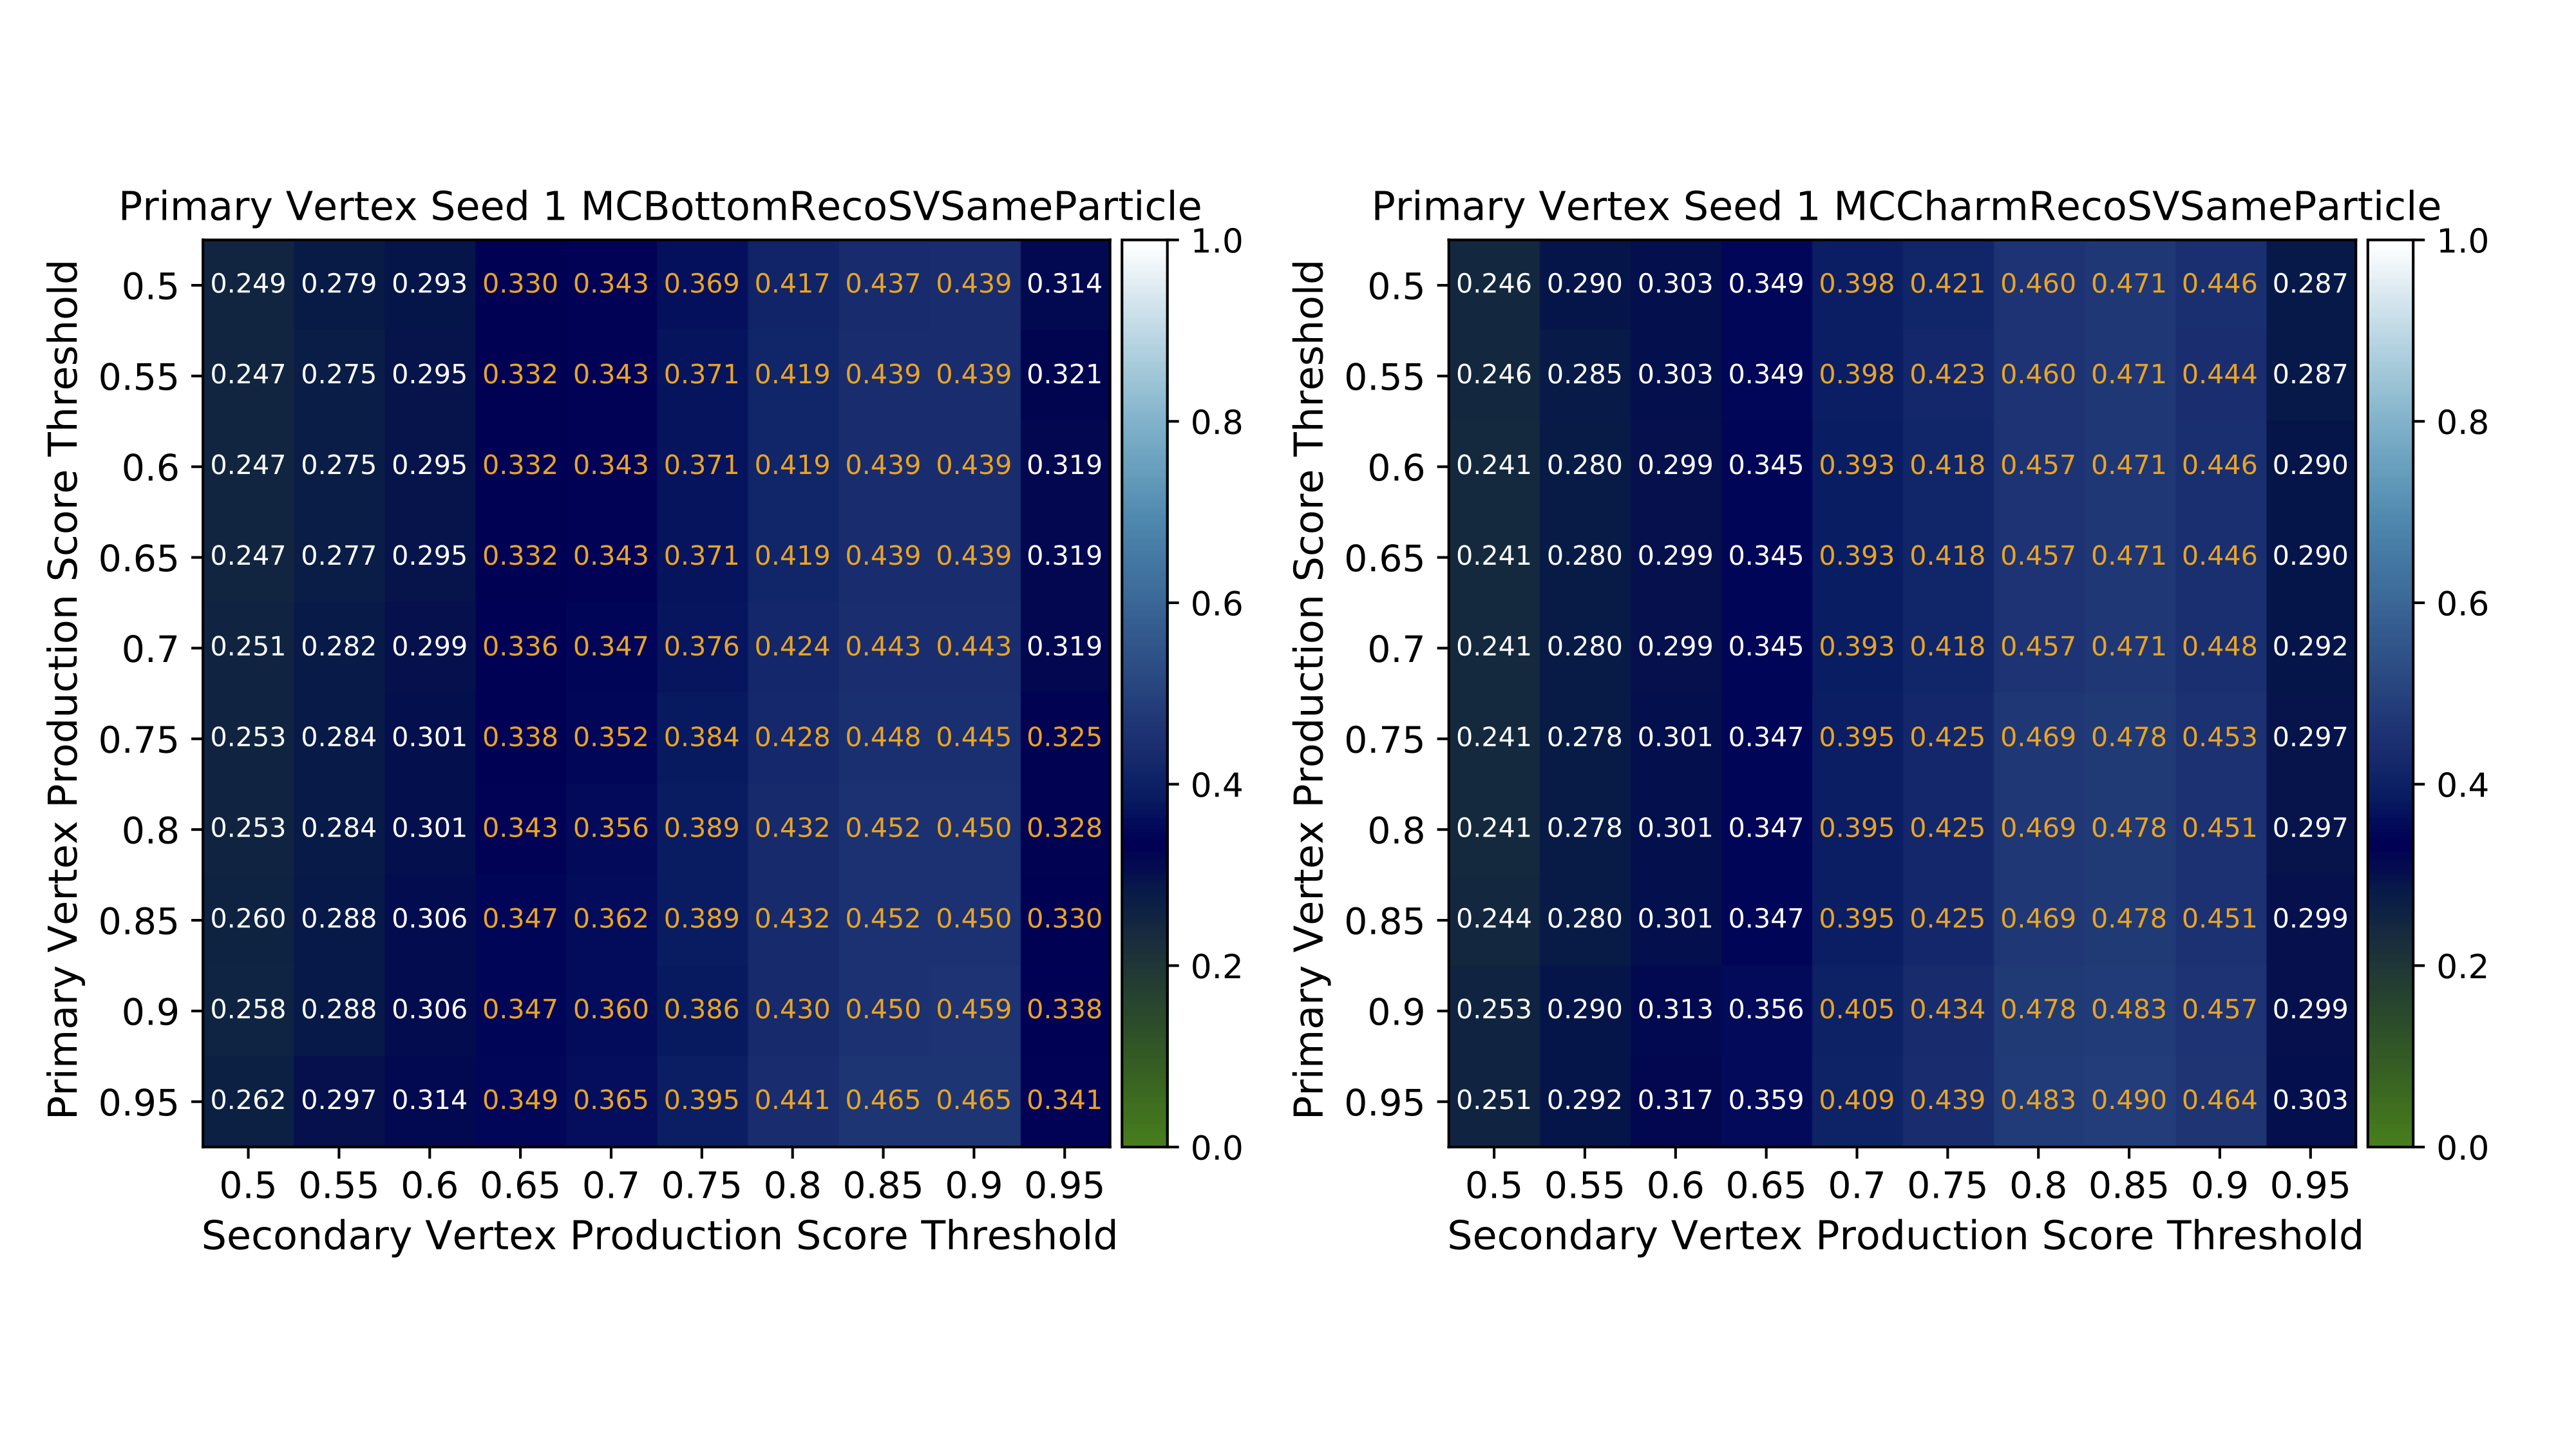
\includegraphics[trim = 0 140 0 140, width=0.95\textwidth, clip]{Figure/4VertexFinderwithDL/4-2-2-2TrackEfficiencySameParticle.png}
   \end{minipage} 
  \caption{閾値と崩壊点検出の性能の関係-PVのタネ1個}
  \label{4-2-2-2TrackEfficiency}
 %\end{tabular}
\end{figure}

\begin{figure}[htbp]
 \centering
  %\begin{tabular}{cccc}
  \begin{minipage}{1.0\textwidth}
   \centering
    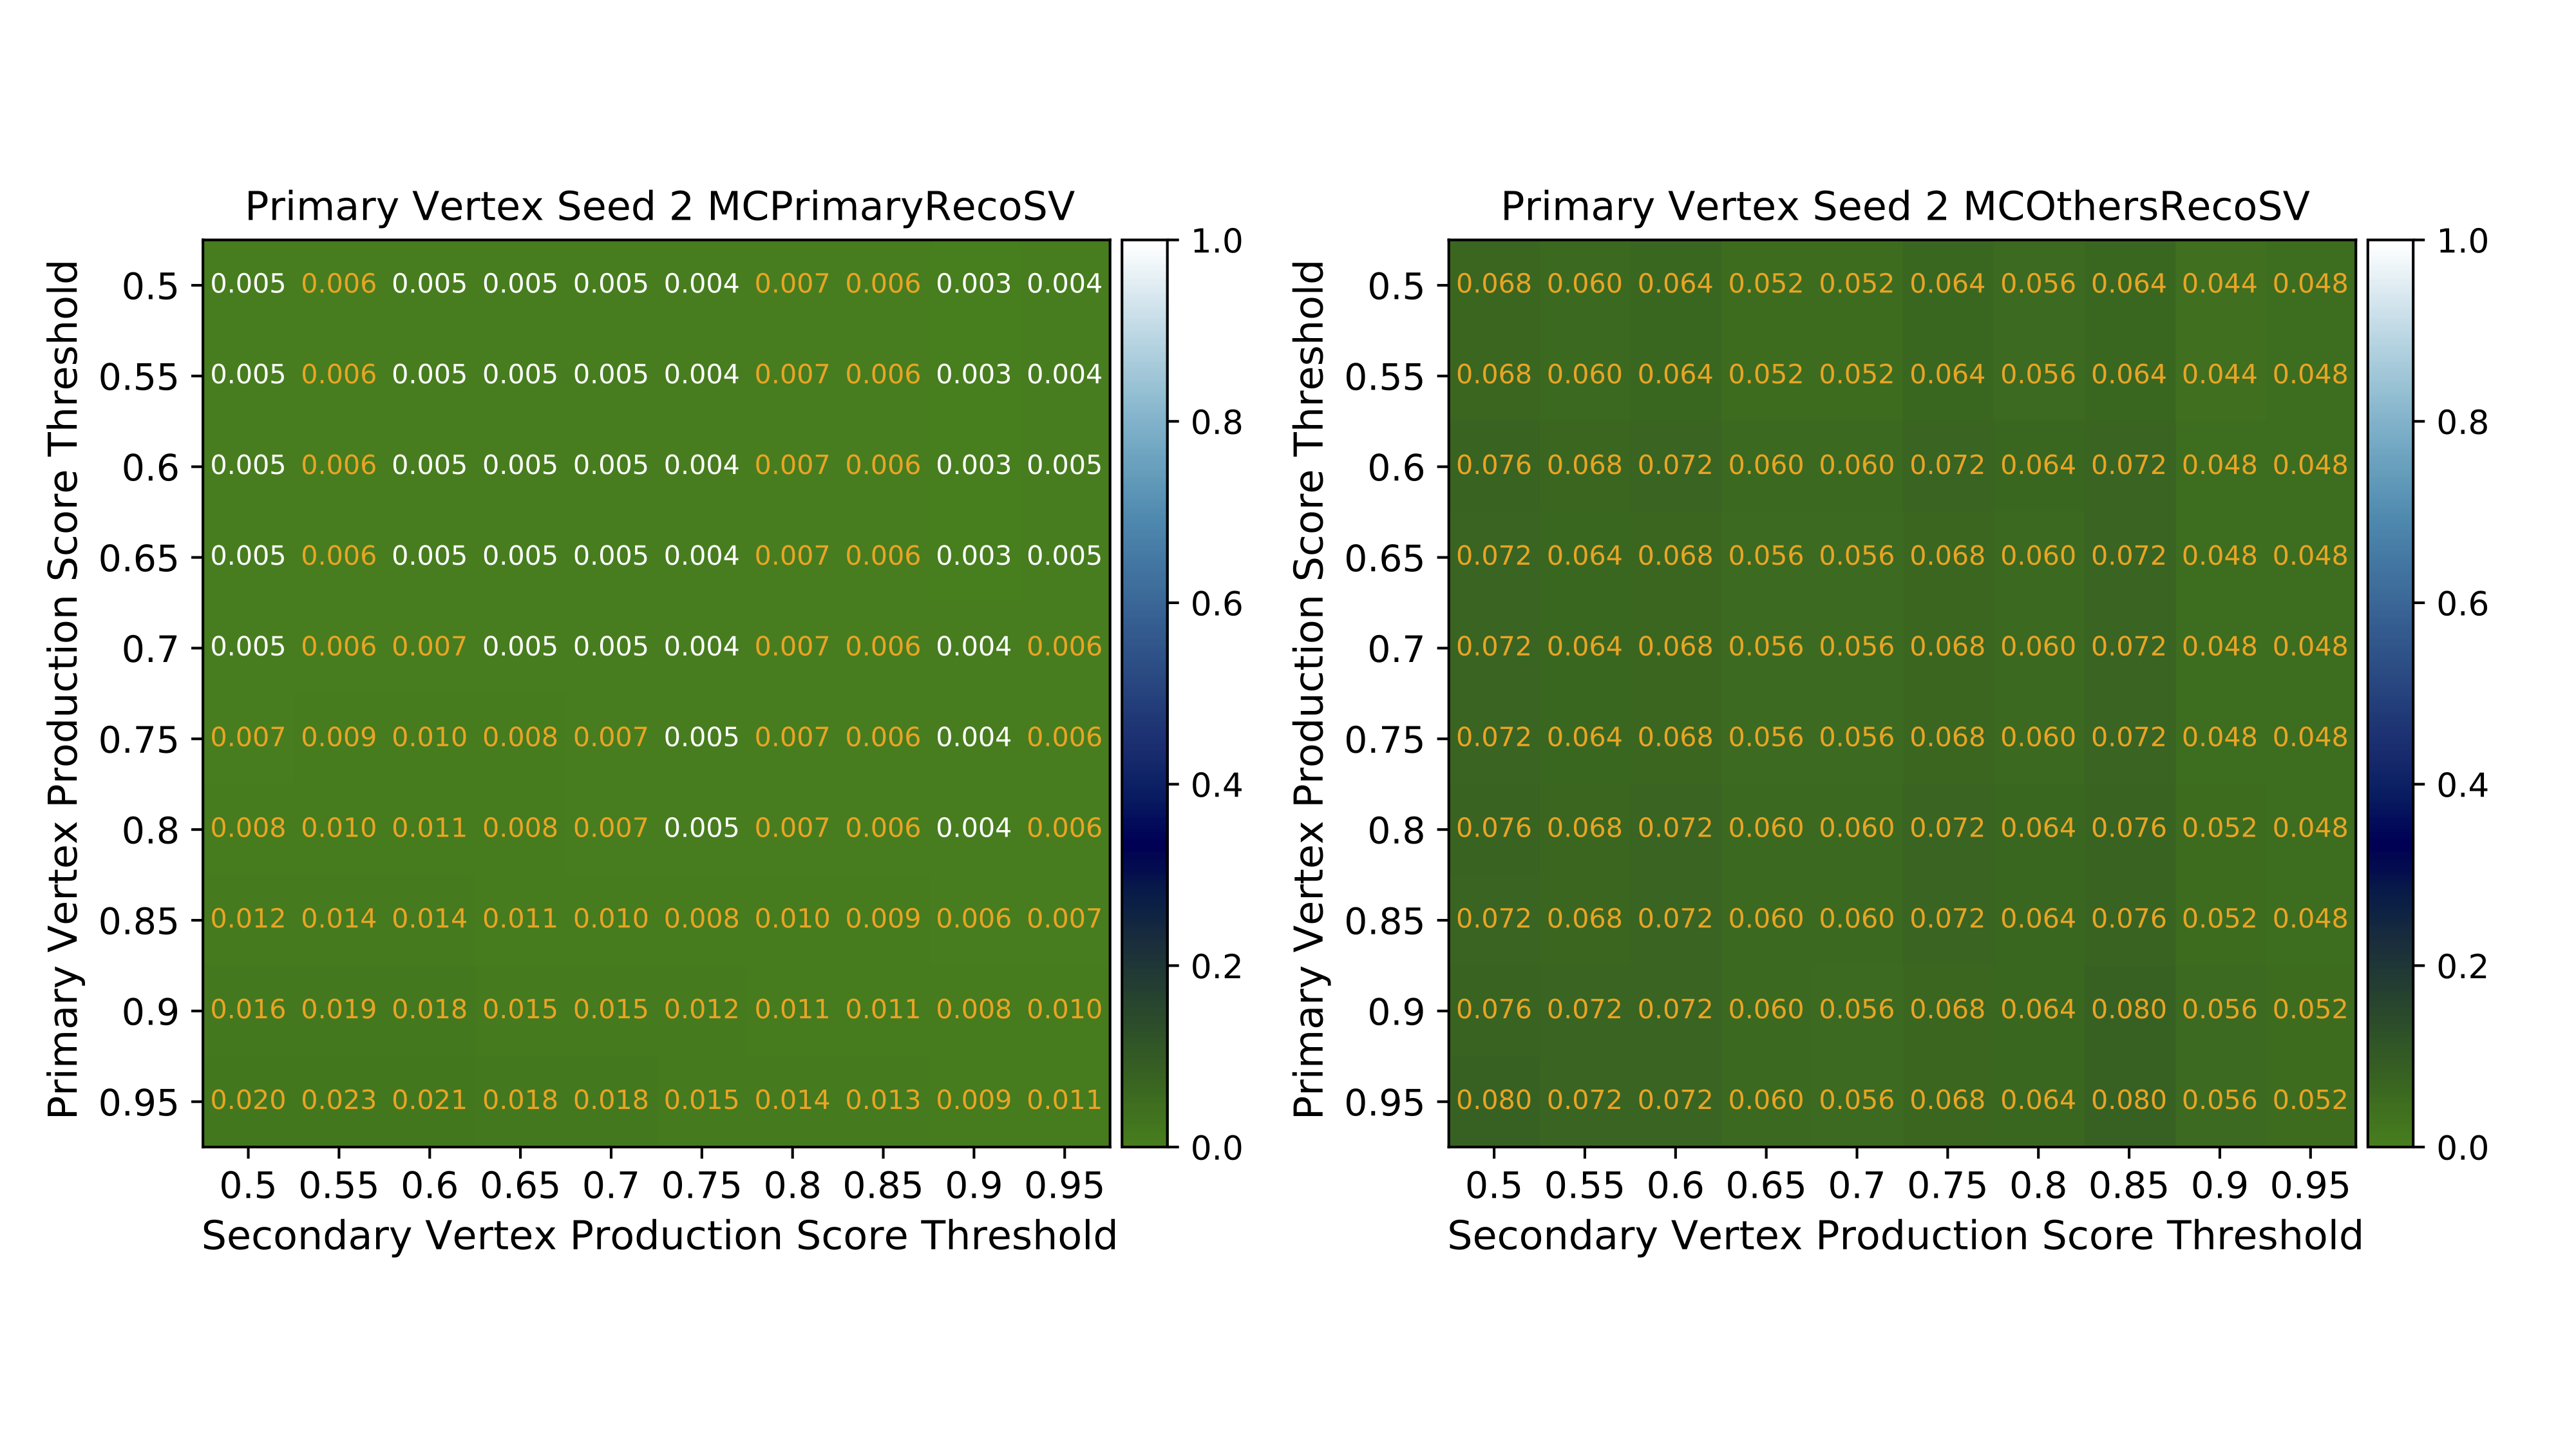
\includegraphics[trim = 0 140 0 140, width=0.95\textwidth, clip]{Figure/4VertexFinderwithDL/4-2-2-3TrackEfficiencyPVOthers.png}
   \end{minipage}
   
   \begin{minipage}{1.0\textwidth}
   \centering
    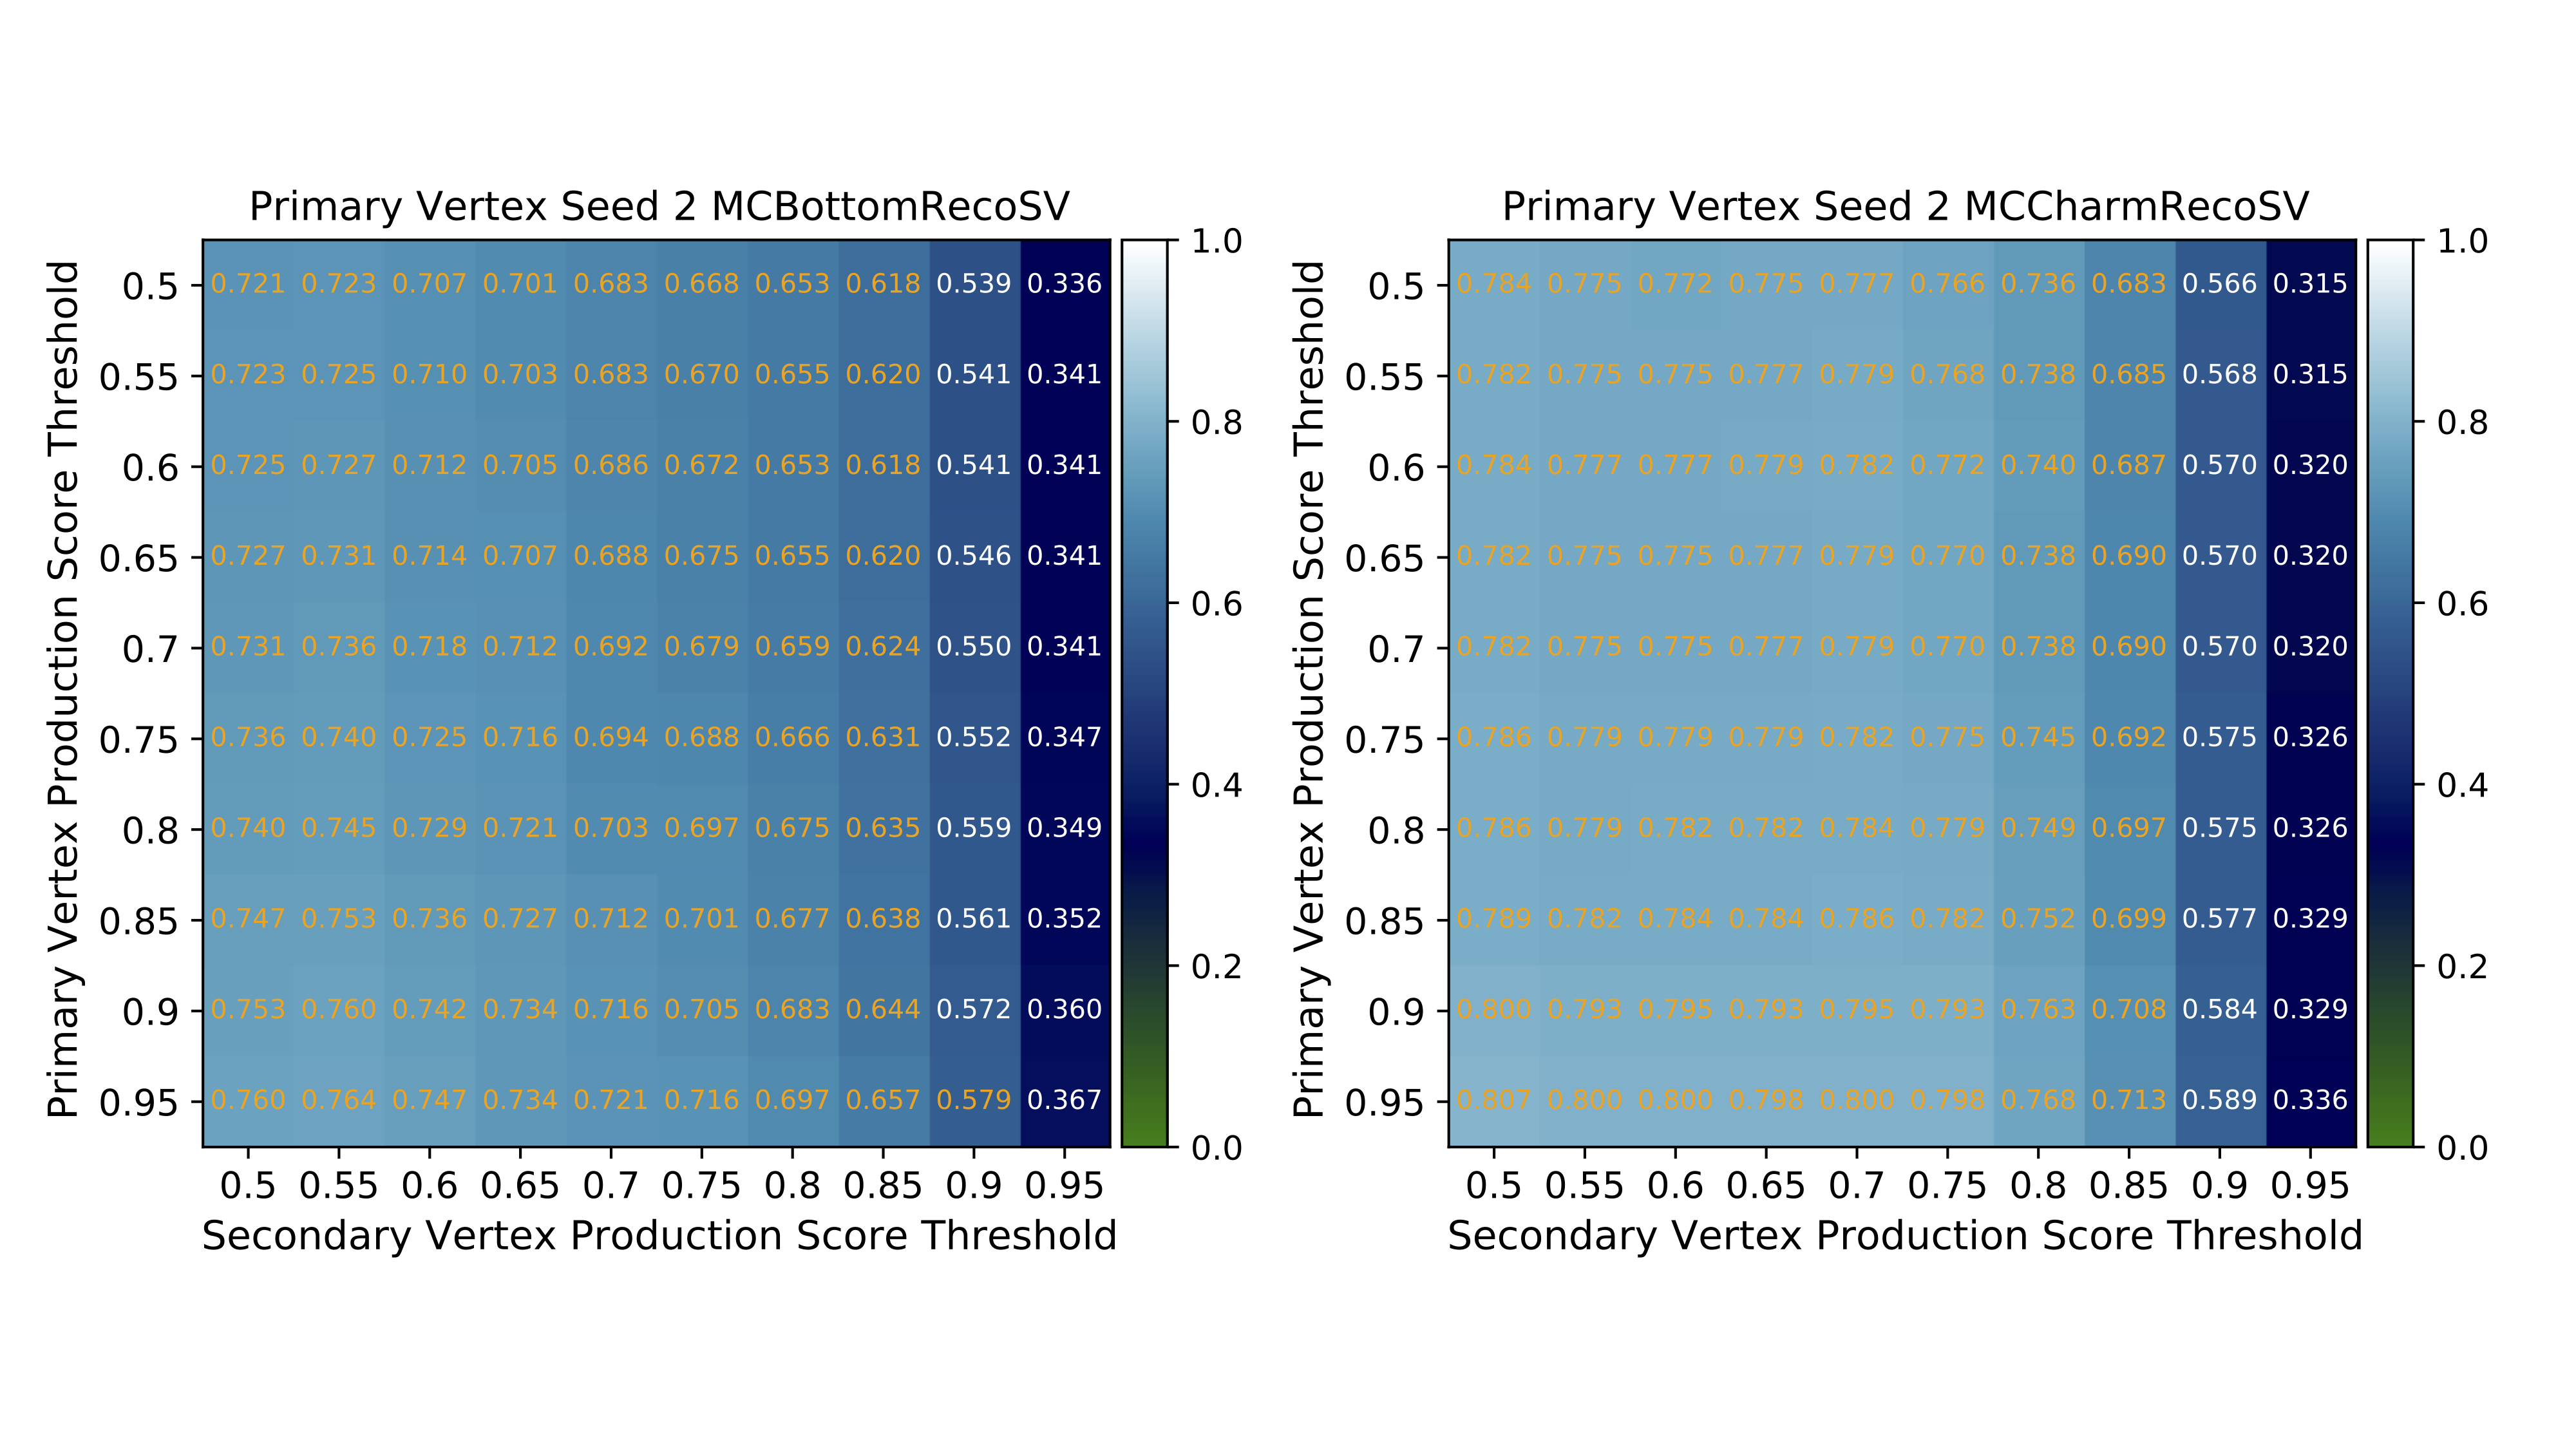
\includegraphics[trim = 0 140 0 140, width=0.95\textwidth, clip]{Figure/4VertexFinderwithDL/4-2-2-3TrackEfficiencyBottomCharm.png}
   \end{minipage}
   
   \begin{minipage}{1.0\textwidth}
   \centering
    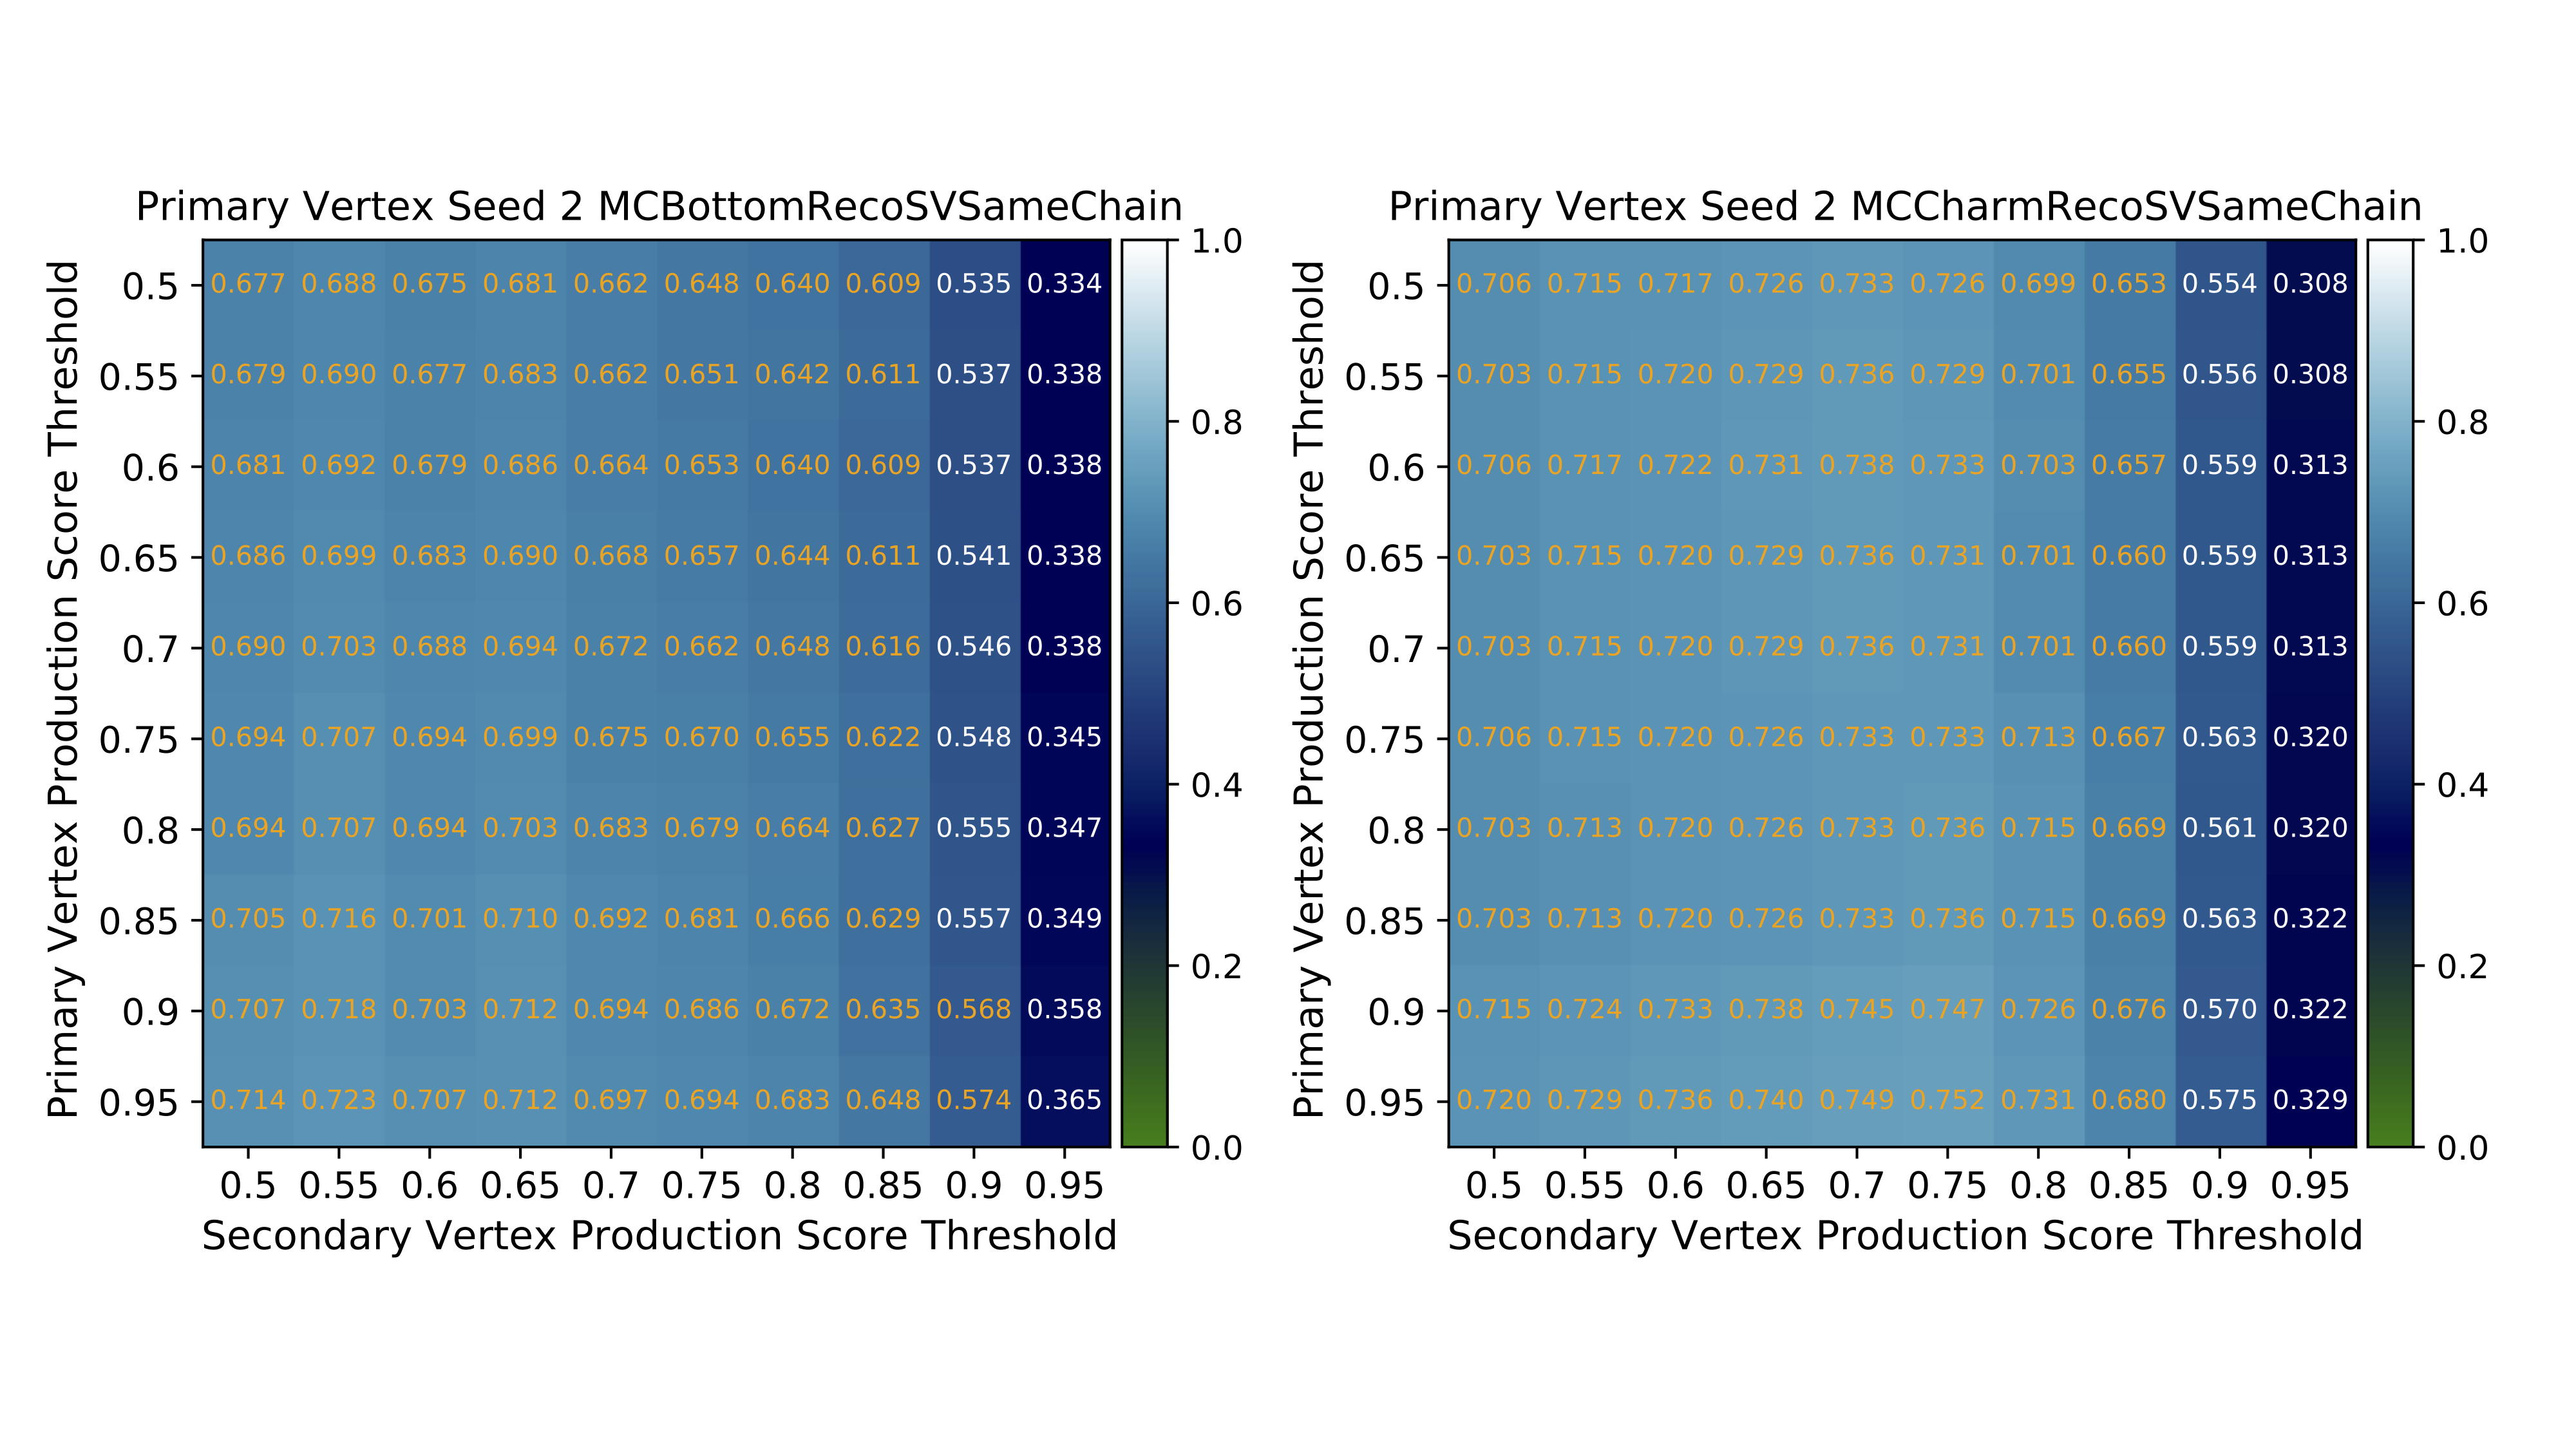
\includegraphics[trim = 0 140 0 140, width=0.95\textwidth, clip]{Figure/4VertexFinderwithDL/4-2-2-3TrackEfficiencySameChain.png}
   \end{minipage}
   
   \begin{minipage}{1.0\textwidth}
   \centering
    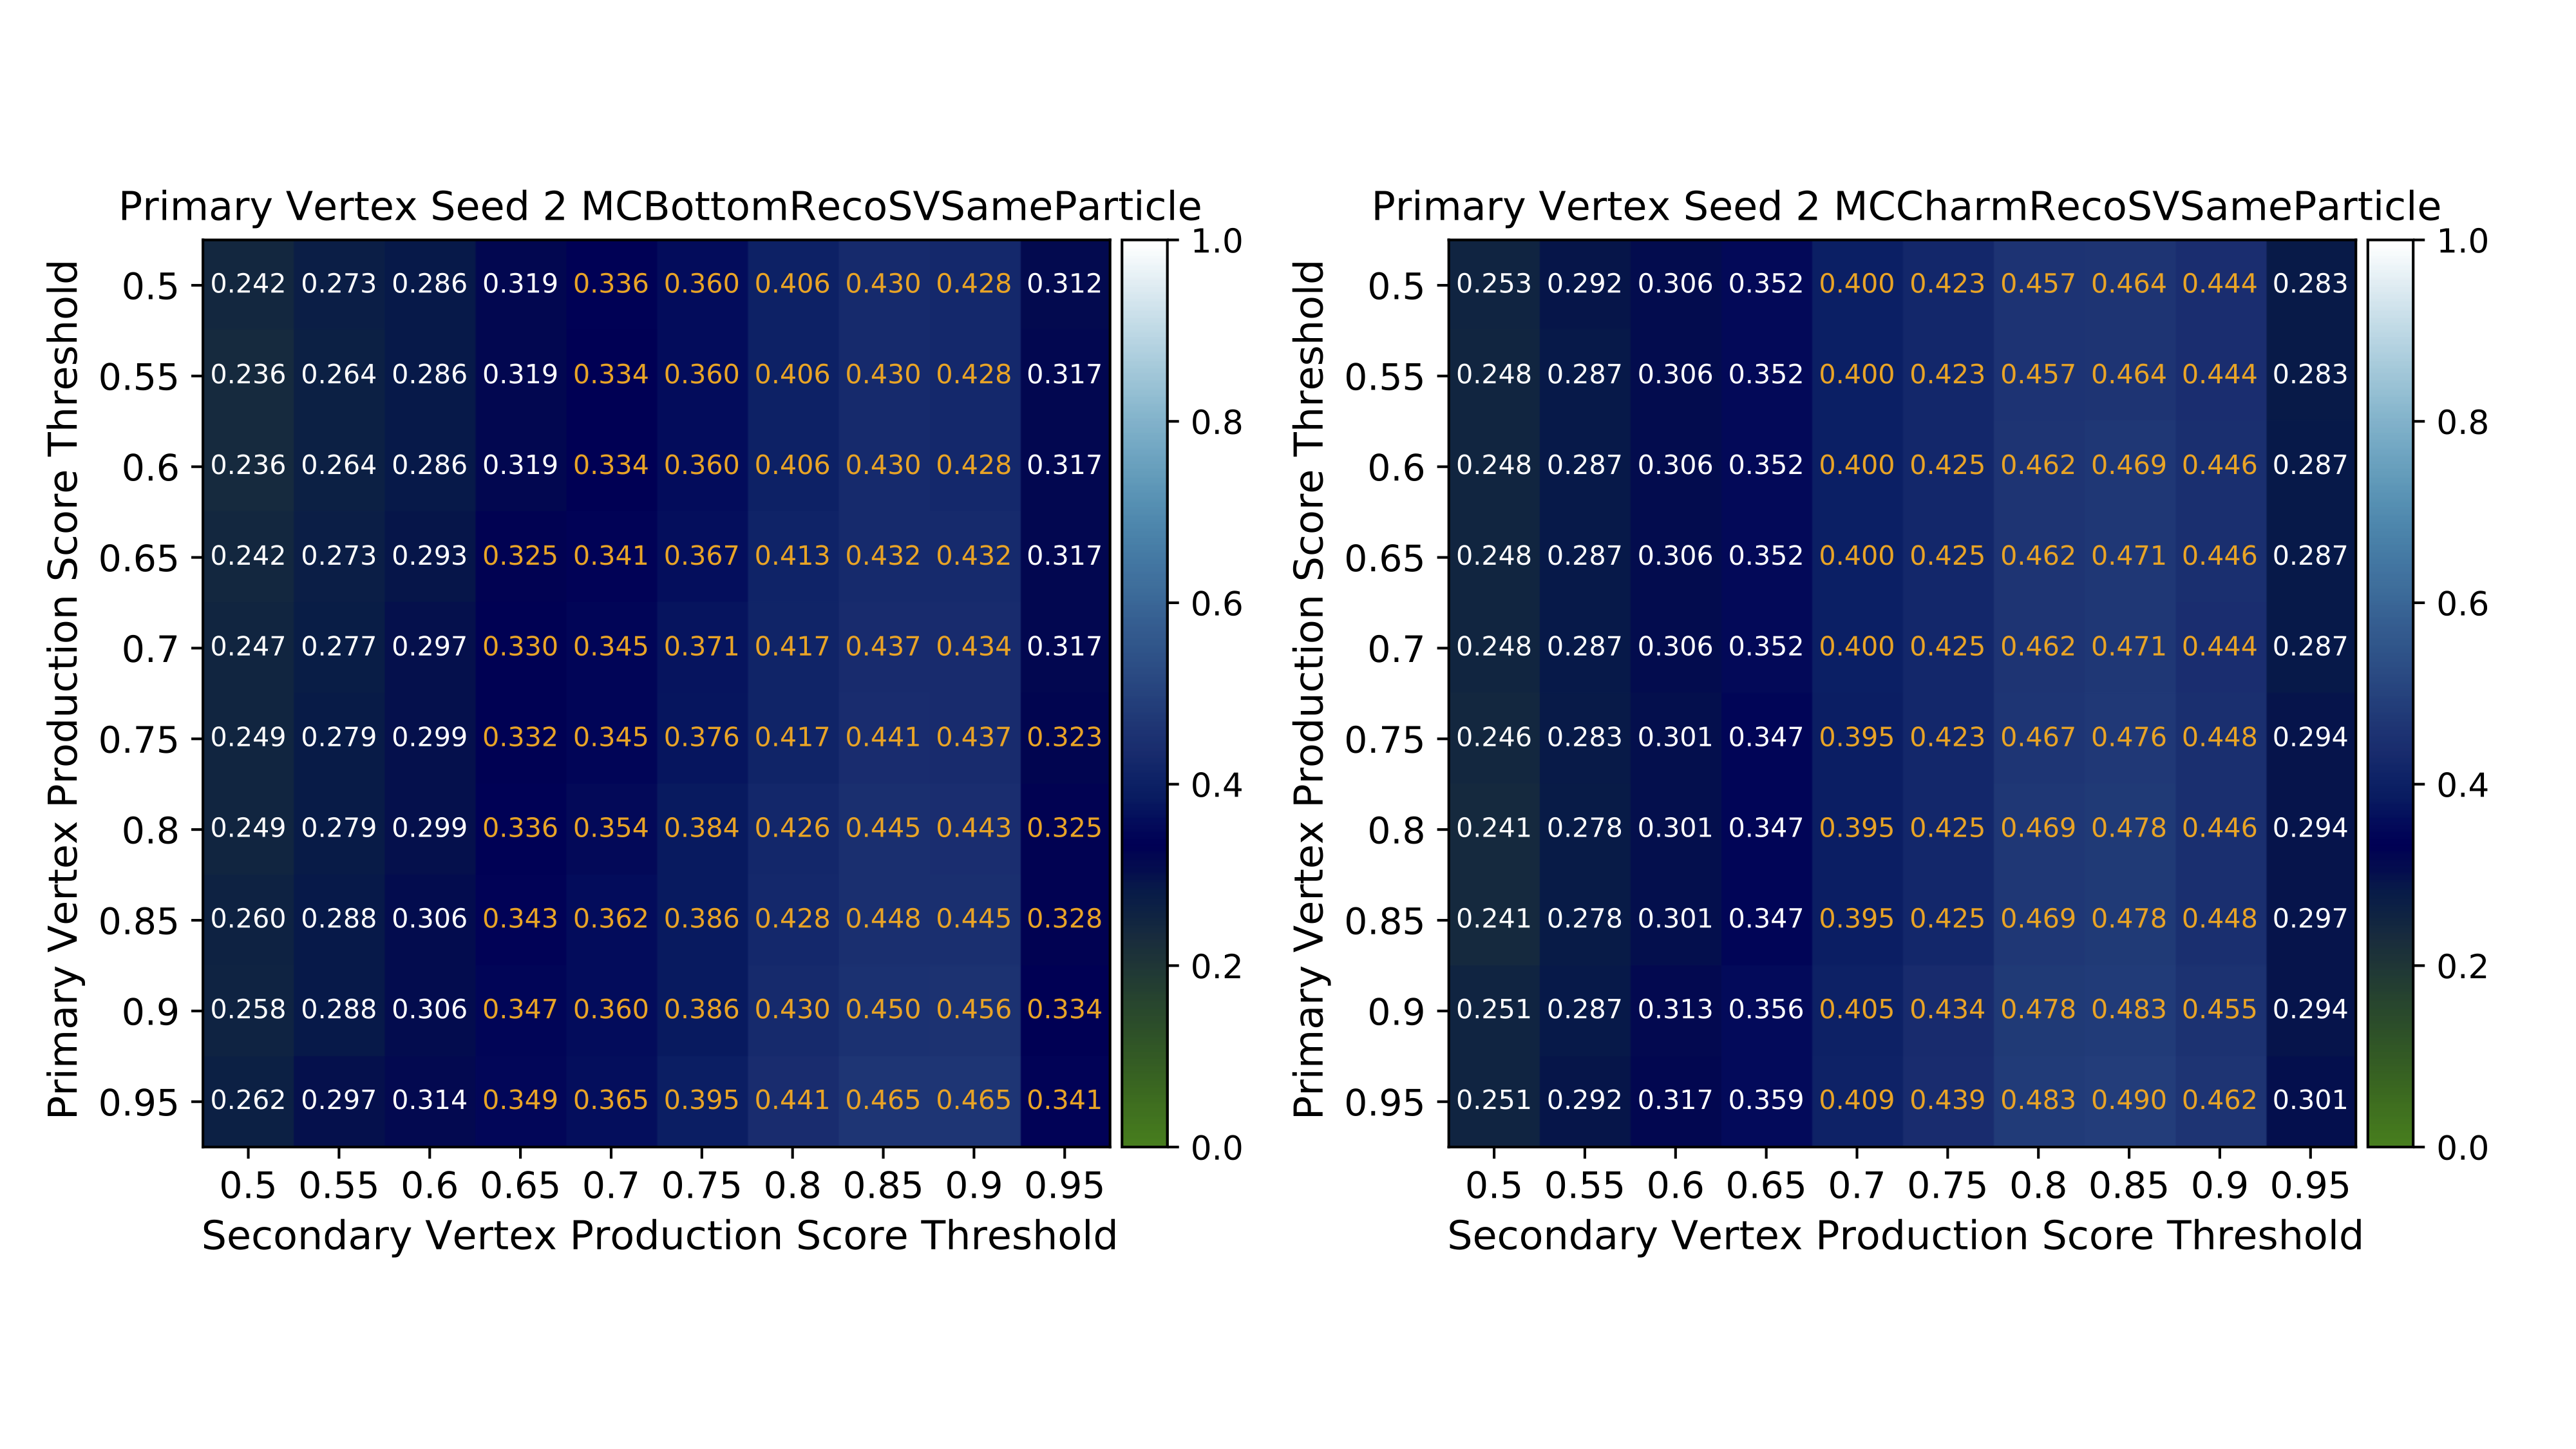
\includegraphics[trim = 0 140 0 140, width=0.95\textwidth, clip]{Figure/4VertexFinderwithDL/4-2-2-3TrackEfficiencySameParticle.png}
   \end{minipage} 
  \caption{閾値と崩壊点検出の性能の関係-PVのタネ2個}
  \label{4-2-2-3TrackEfficiency}
 %\end{tabular}
\end{figure}

\begin{figure}[htbp]
 \centering
  %\begin{tabular}{cccc}
  \begin{minipage}{1.0\textwidth}
   \centering
    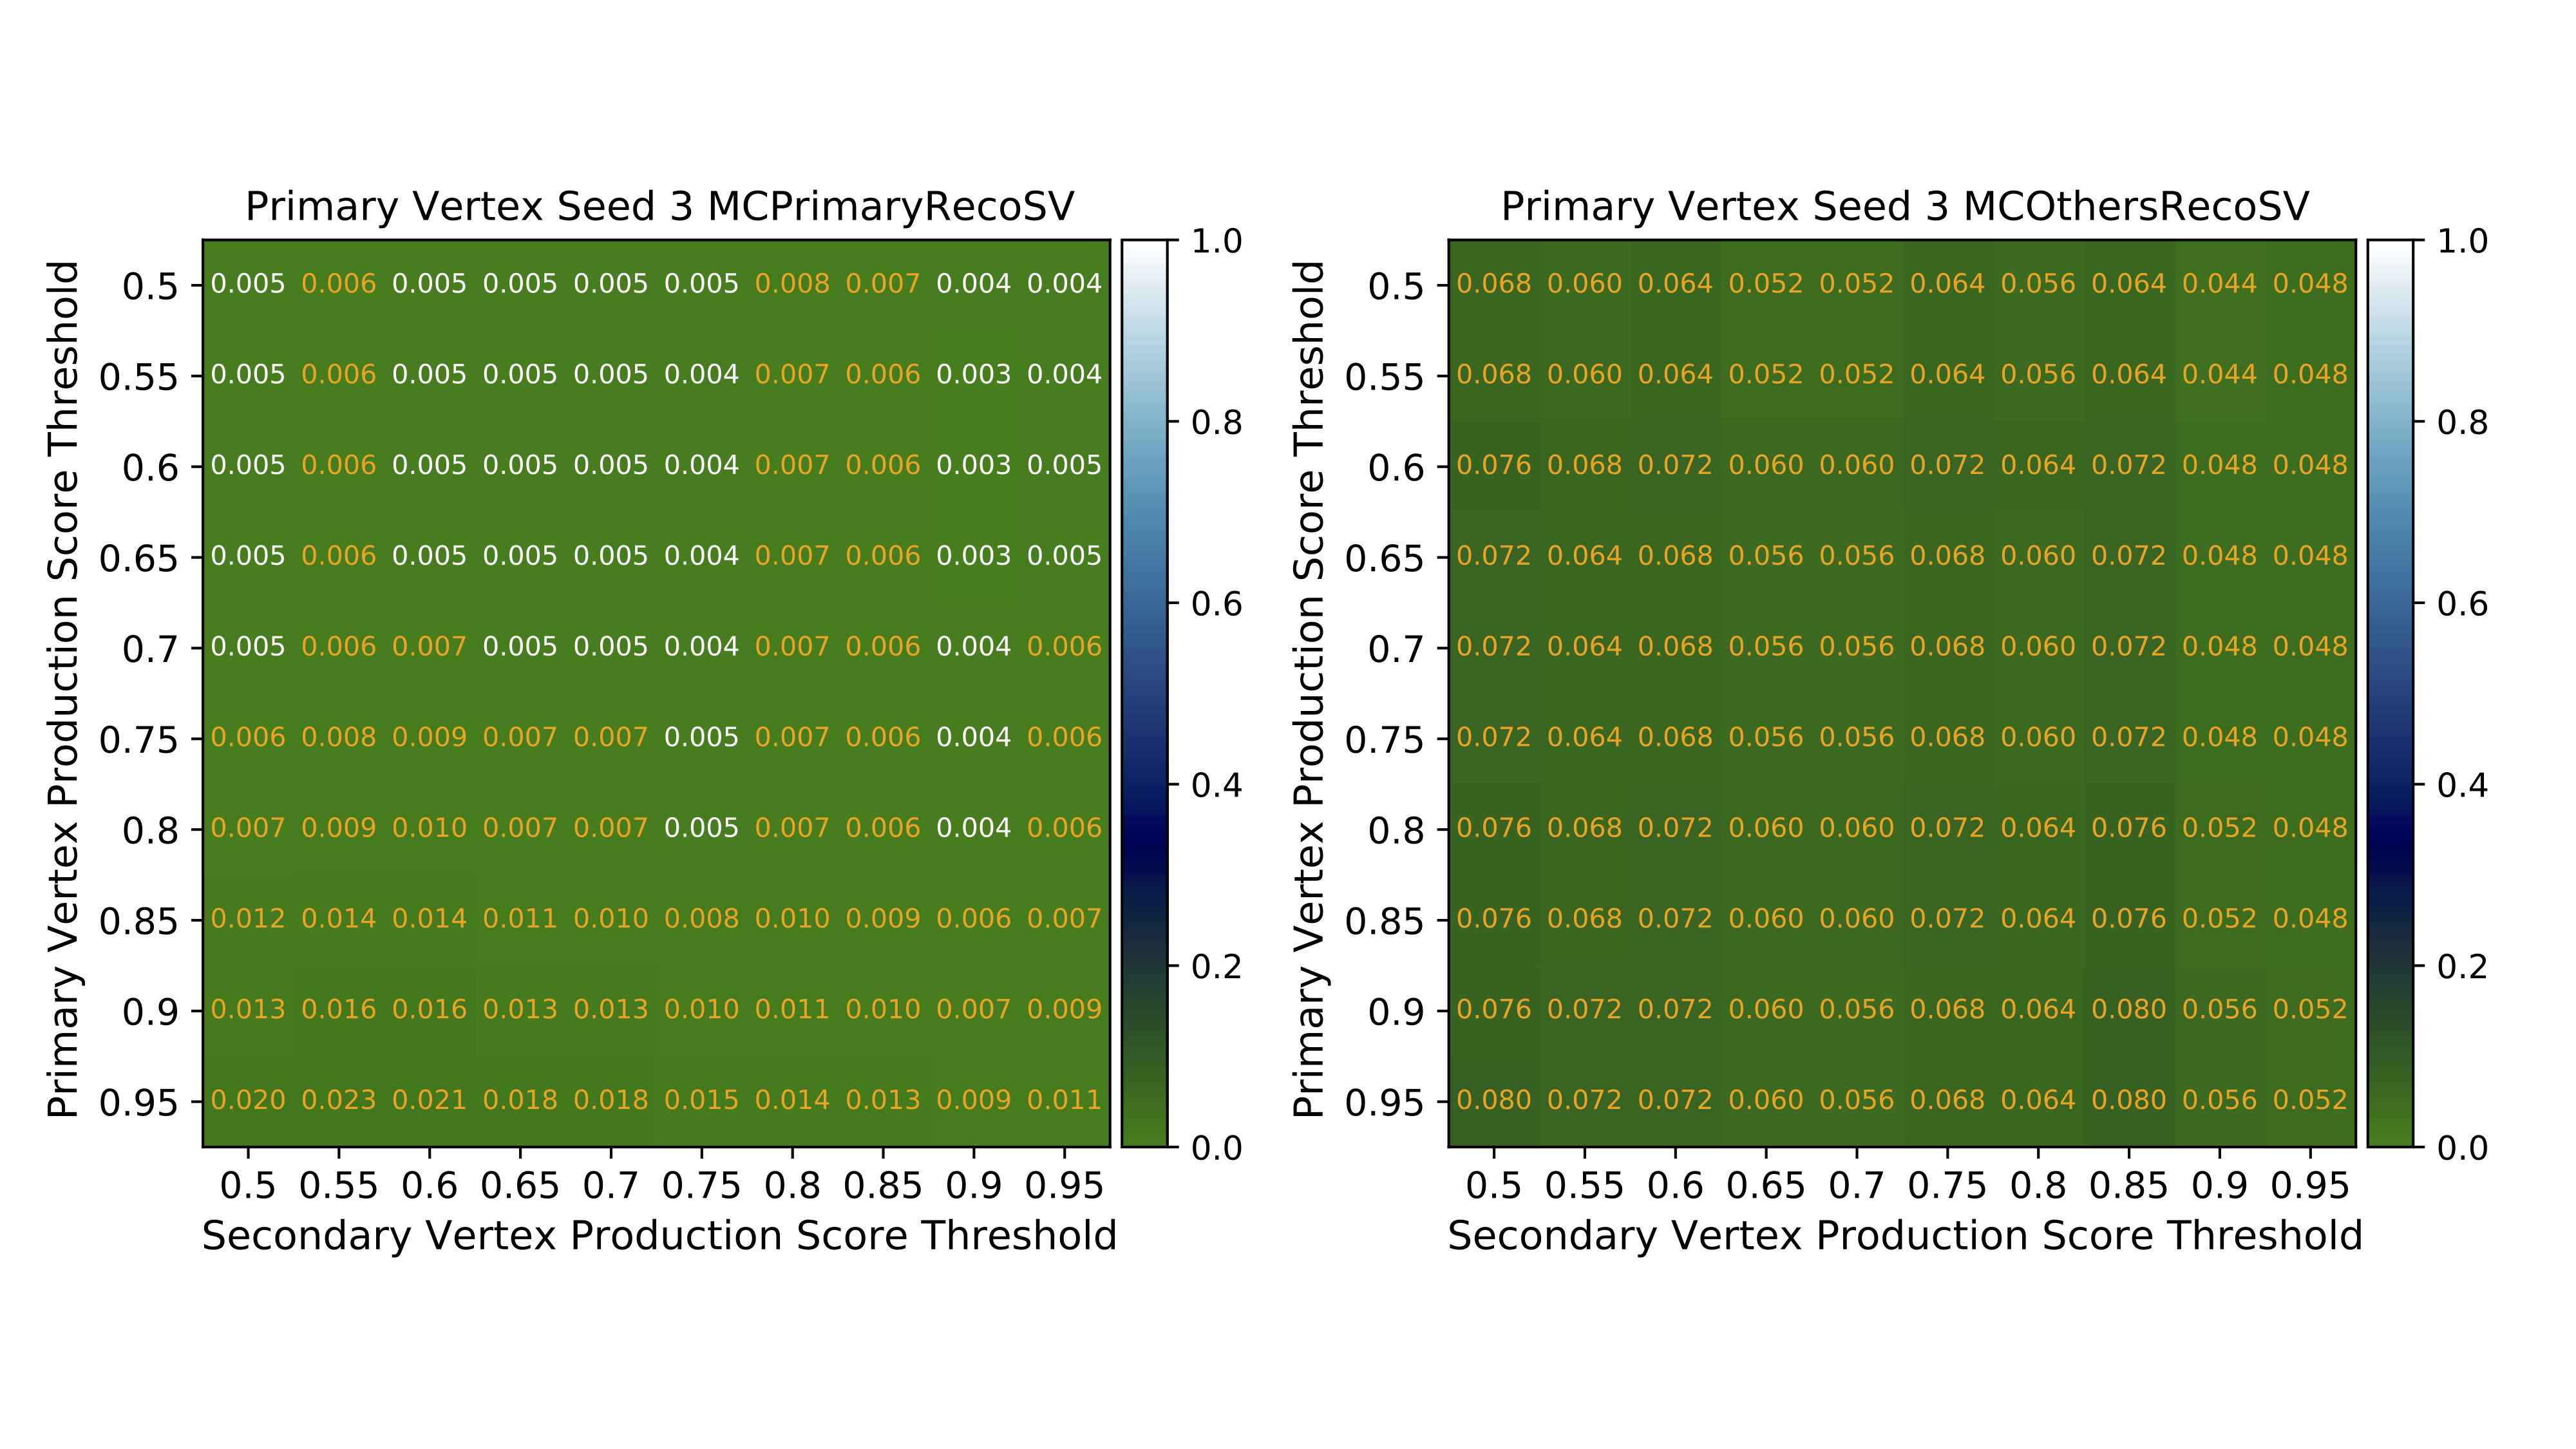
\includegraphics[trim = 0 140 0 140, width=0.95\textwidth, clip]{Figure/4VertexFinderwithDL/4-2-2-4TrackEfficiencyPVOthers.png}
   \end{minipage}
   
   \begin{minipage}{1.0\textwidth}
   \centering
    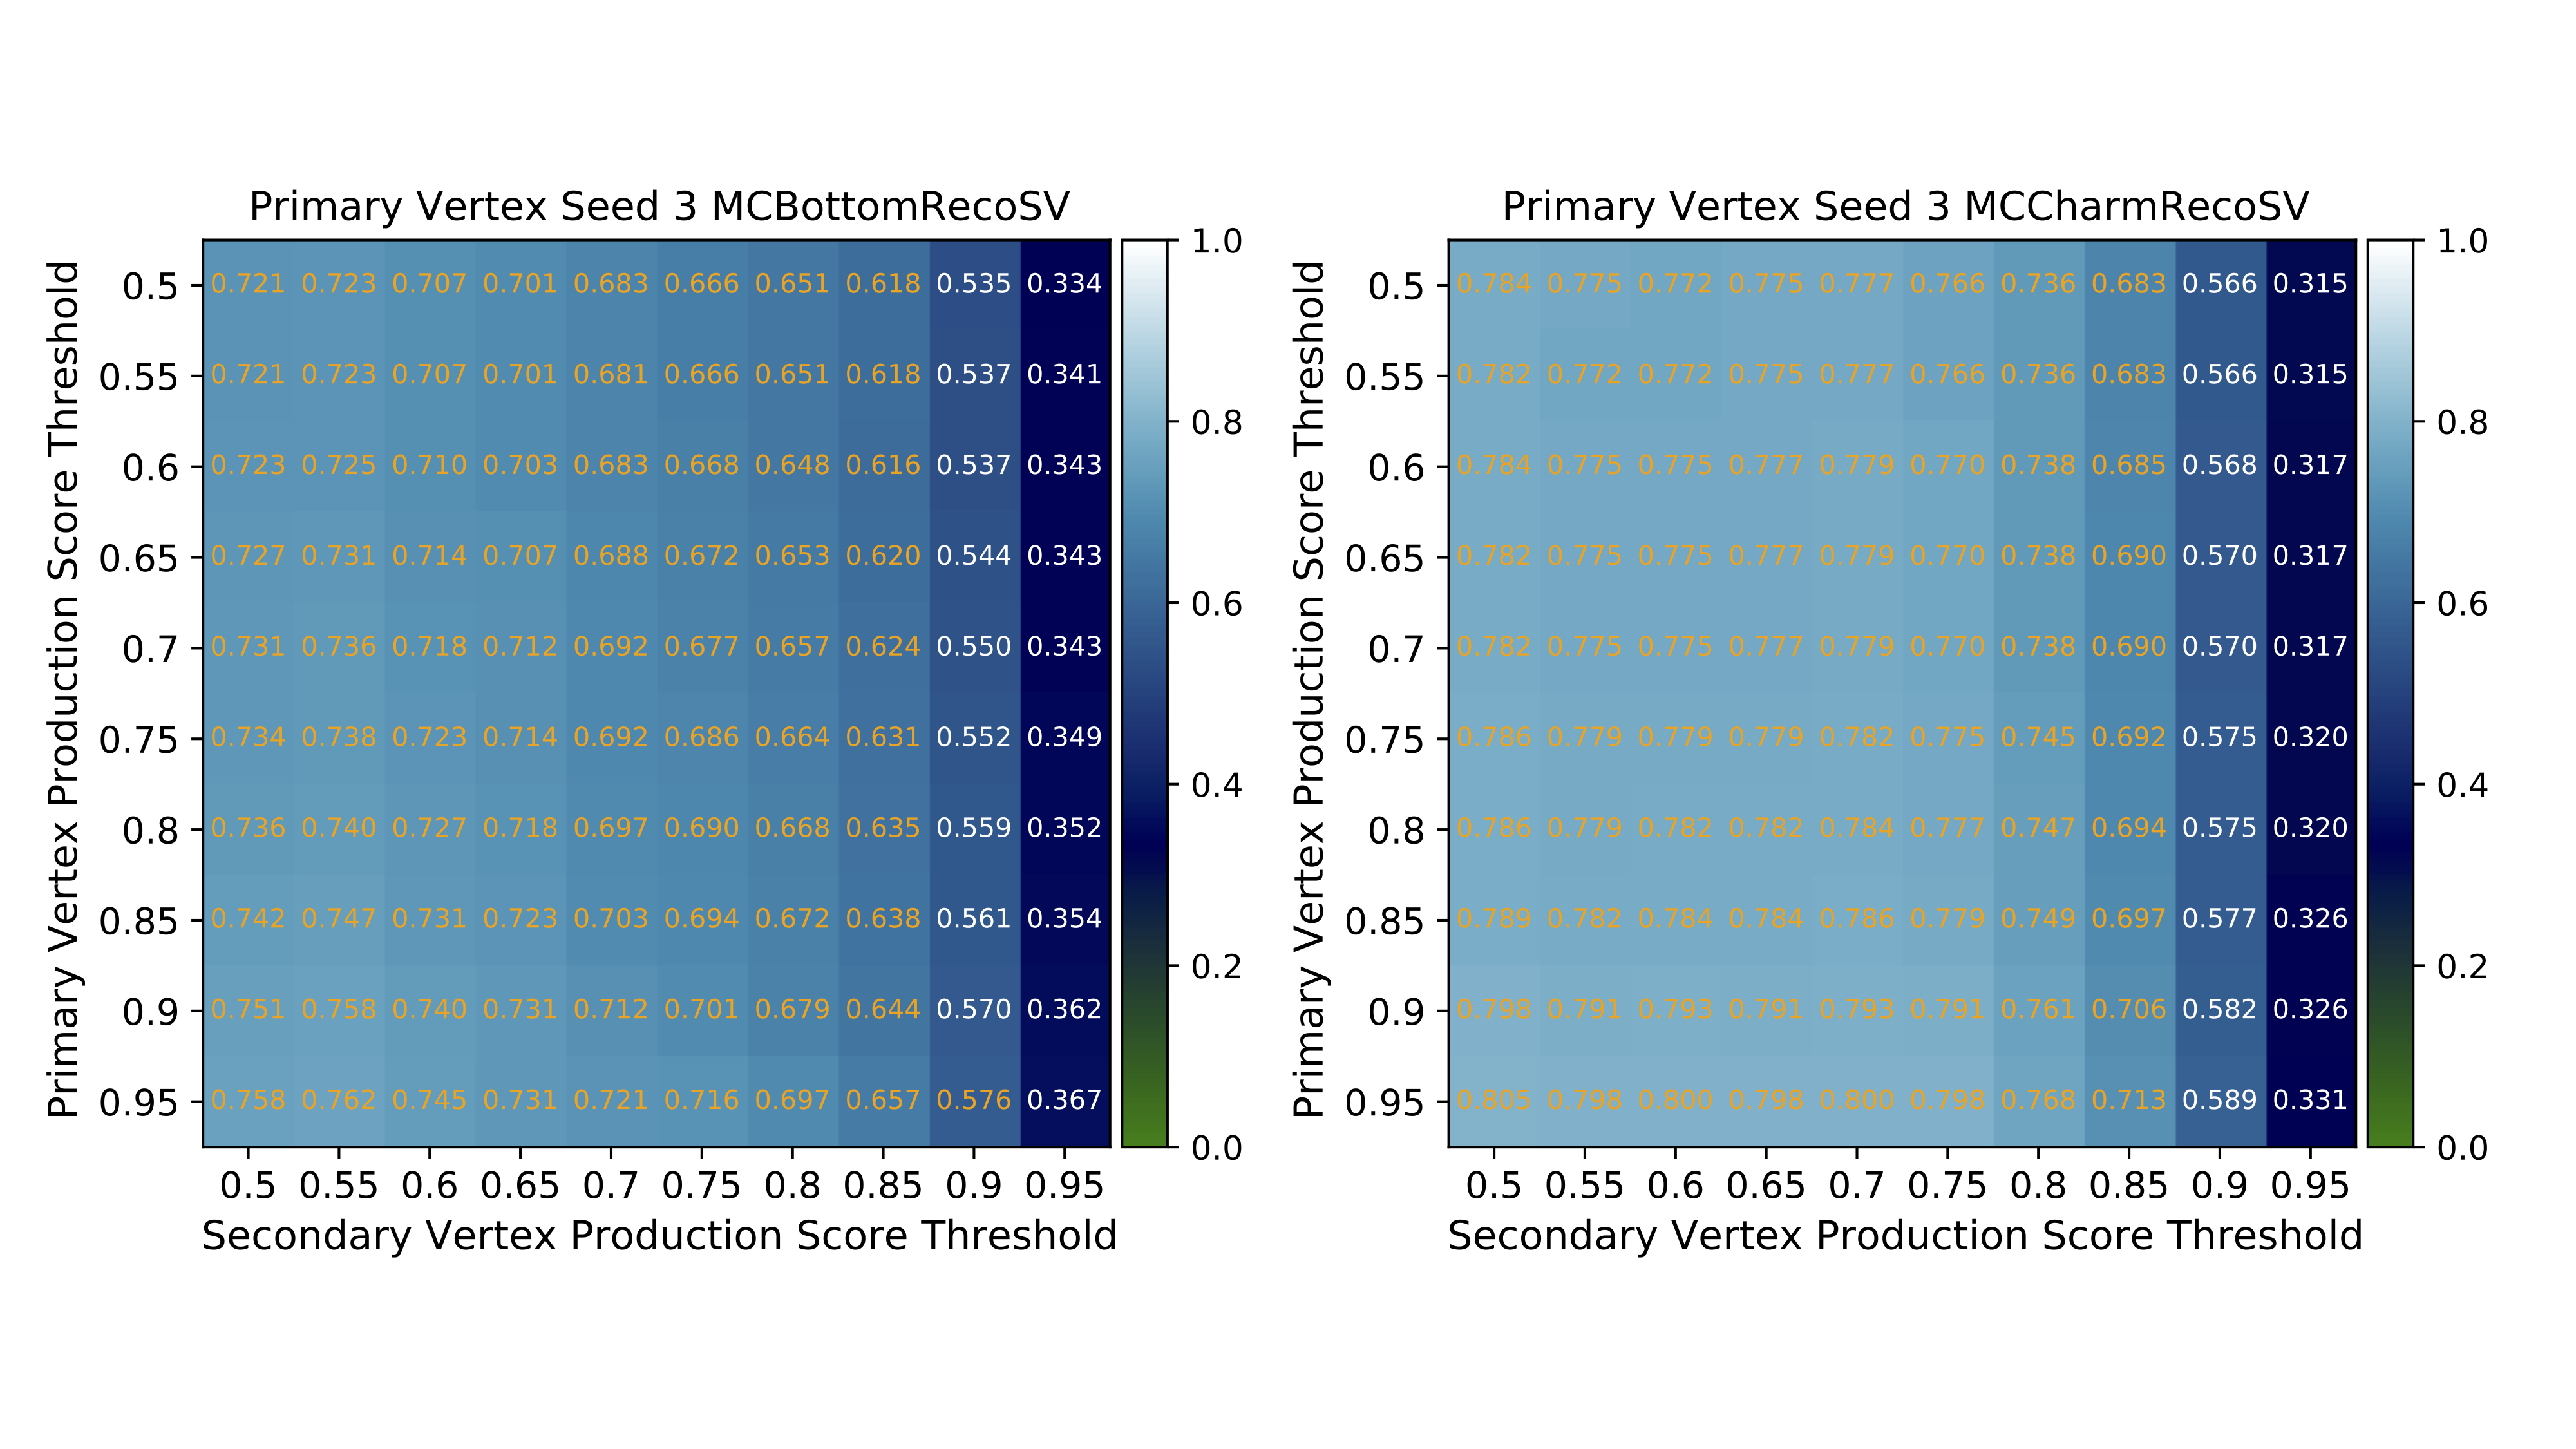
\includegraphics[trim = 0 140 0 140, width=0.95\textwidth, clip]{Figure/4VertexFinderwithDL/4-2-2-4TrackEfficiencyBottomCharm.png}
   \end{minipage}
   
   \begin{minipage}{1.0\textwidth}
   \centering
    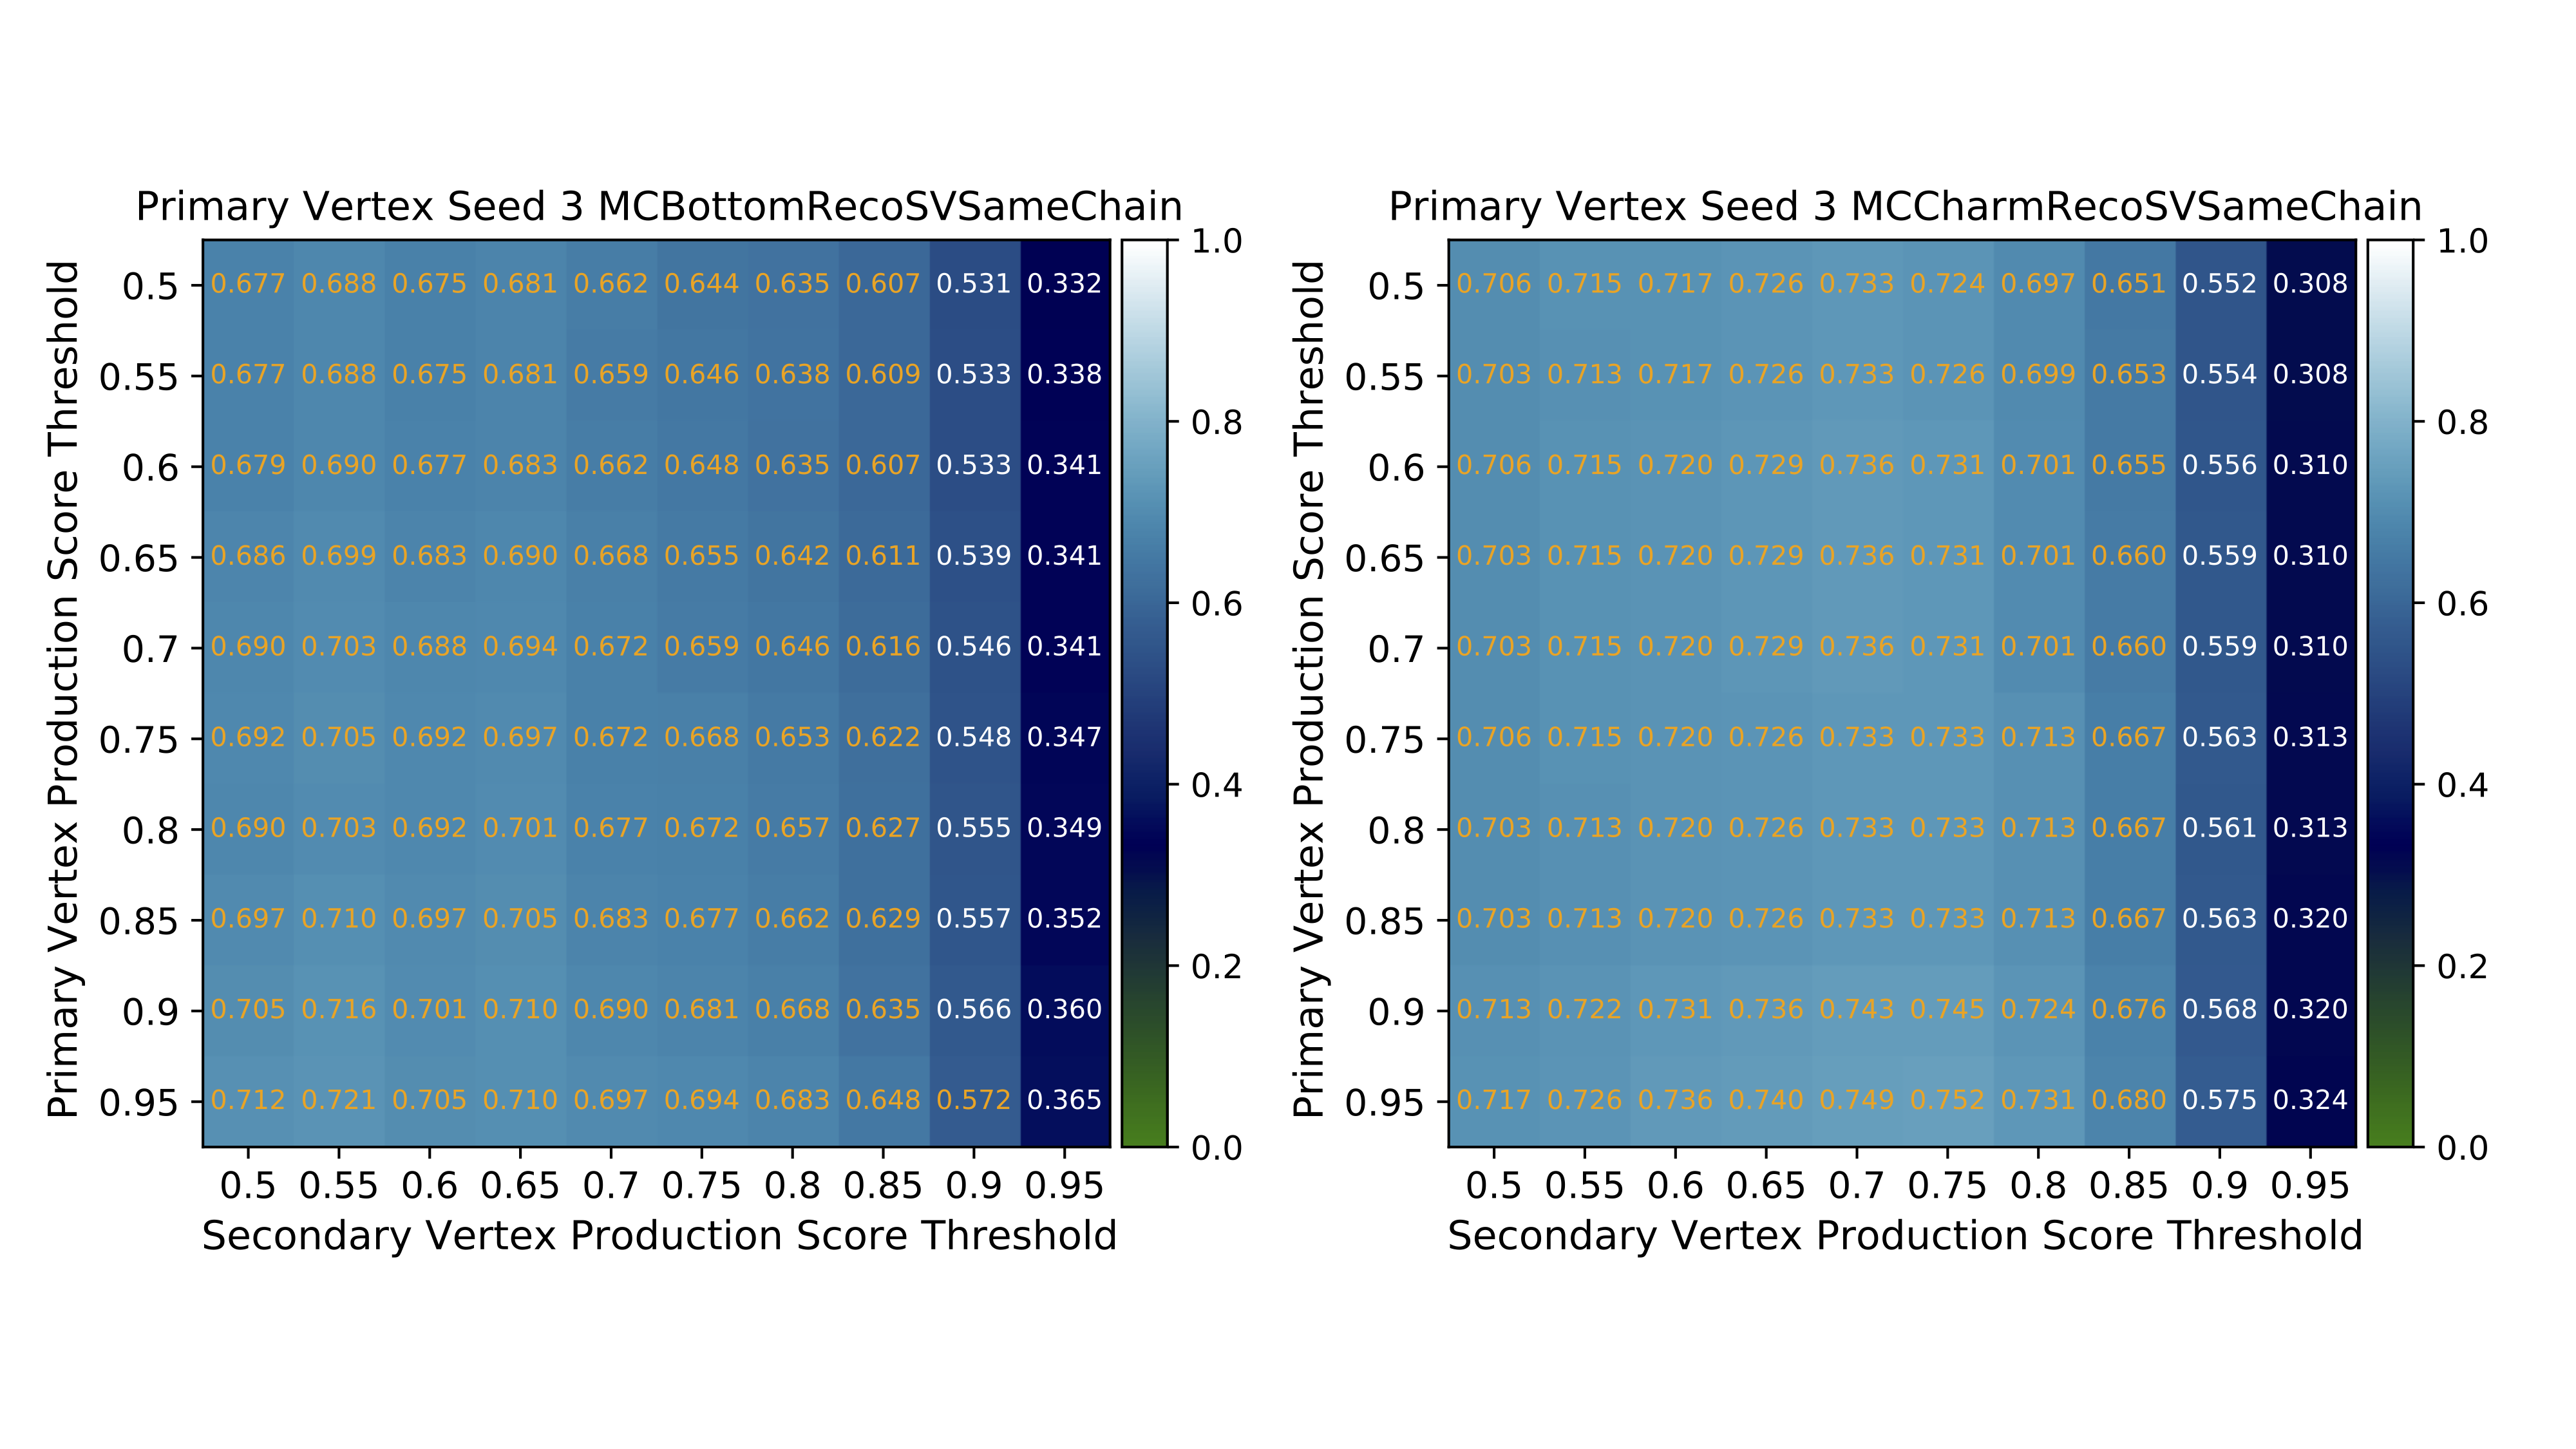
\includegraphics[trim = 0 140 0 140, width=0.95\textwidth, clip]{Figure/4VertexFinderwithDL/4-2-2-4TrackEfficiencySameChain.png}
   \end{minipage}
   
   \begin{minipage}{1.0\textwidth}
   \centering
    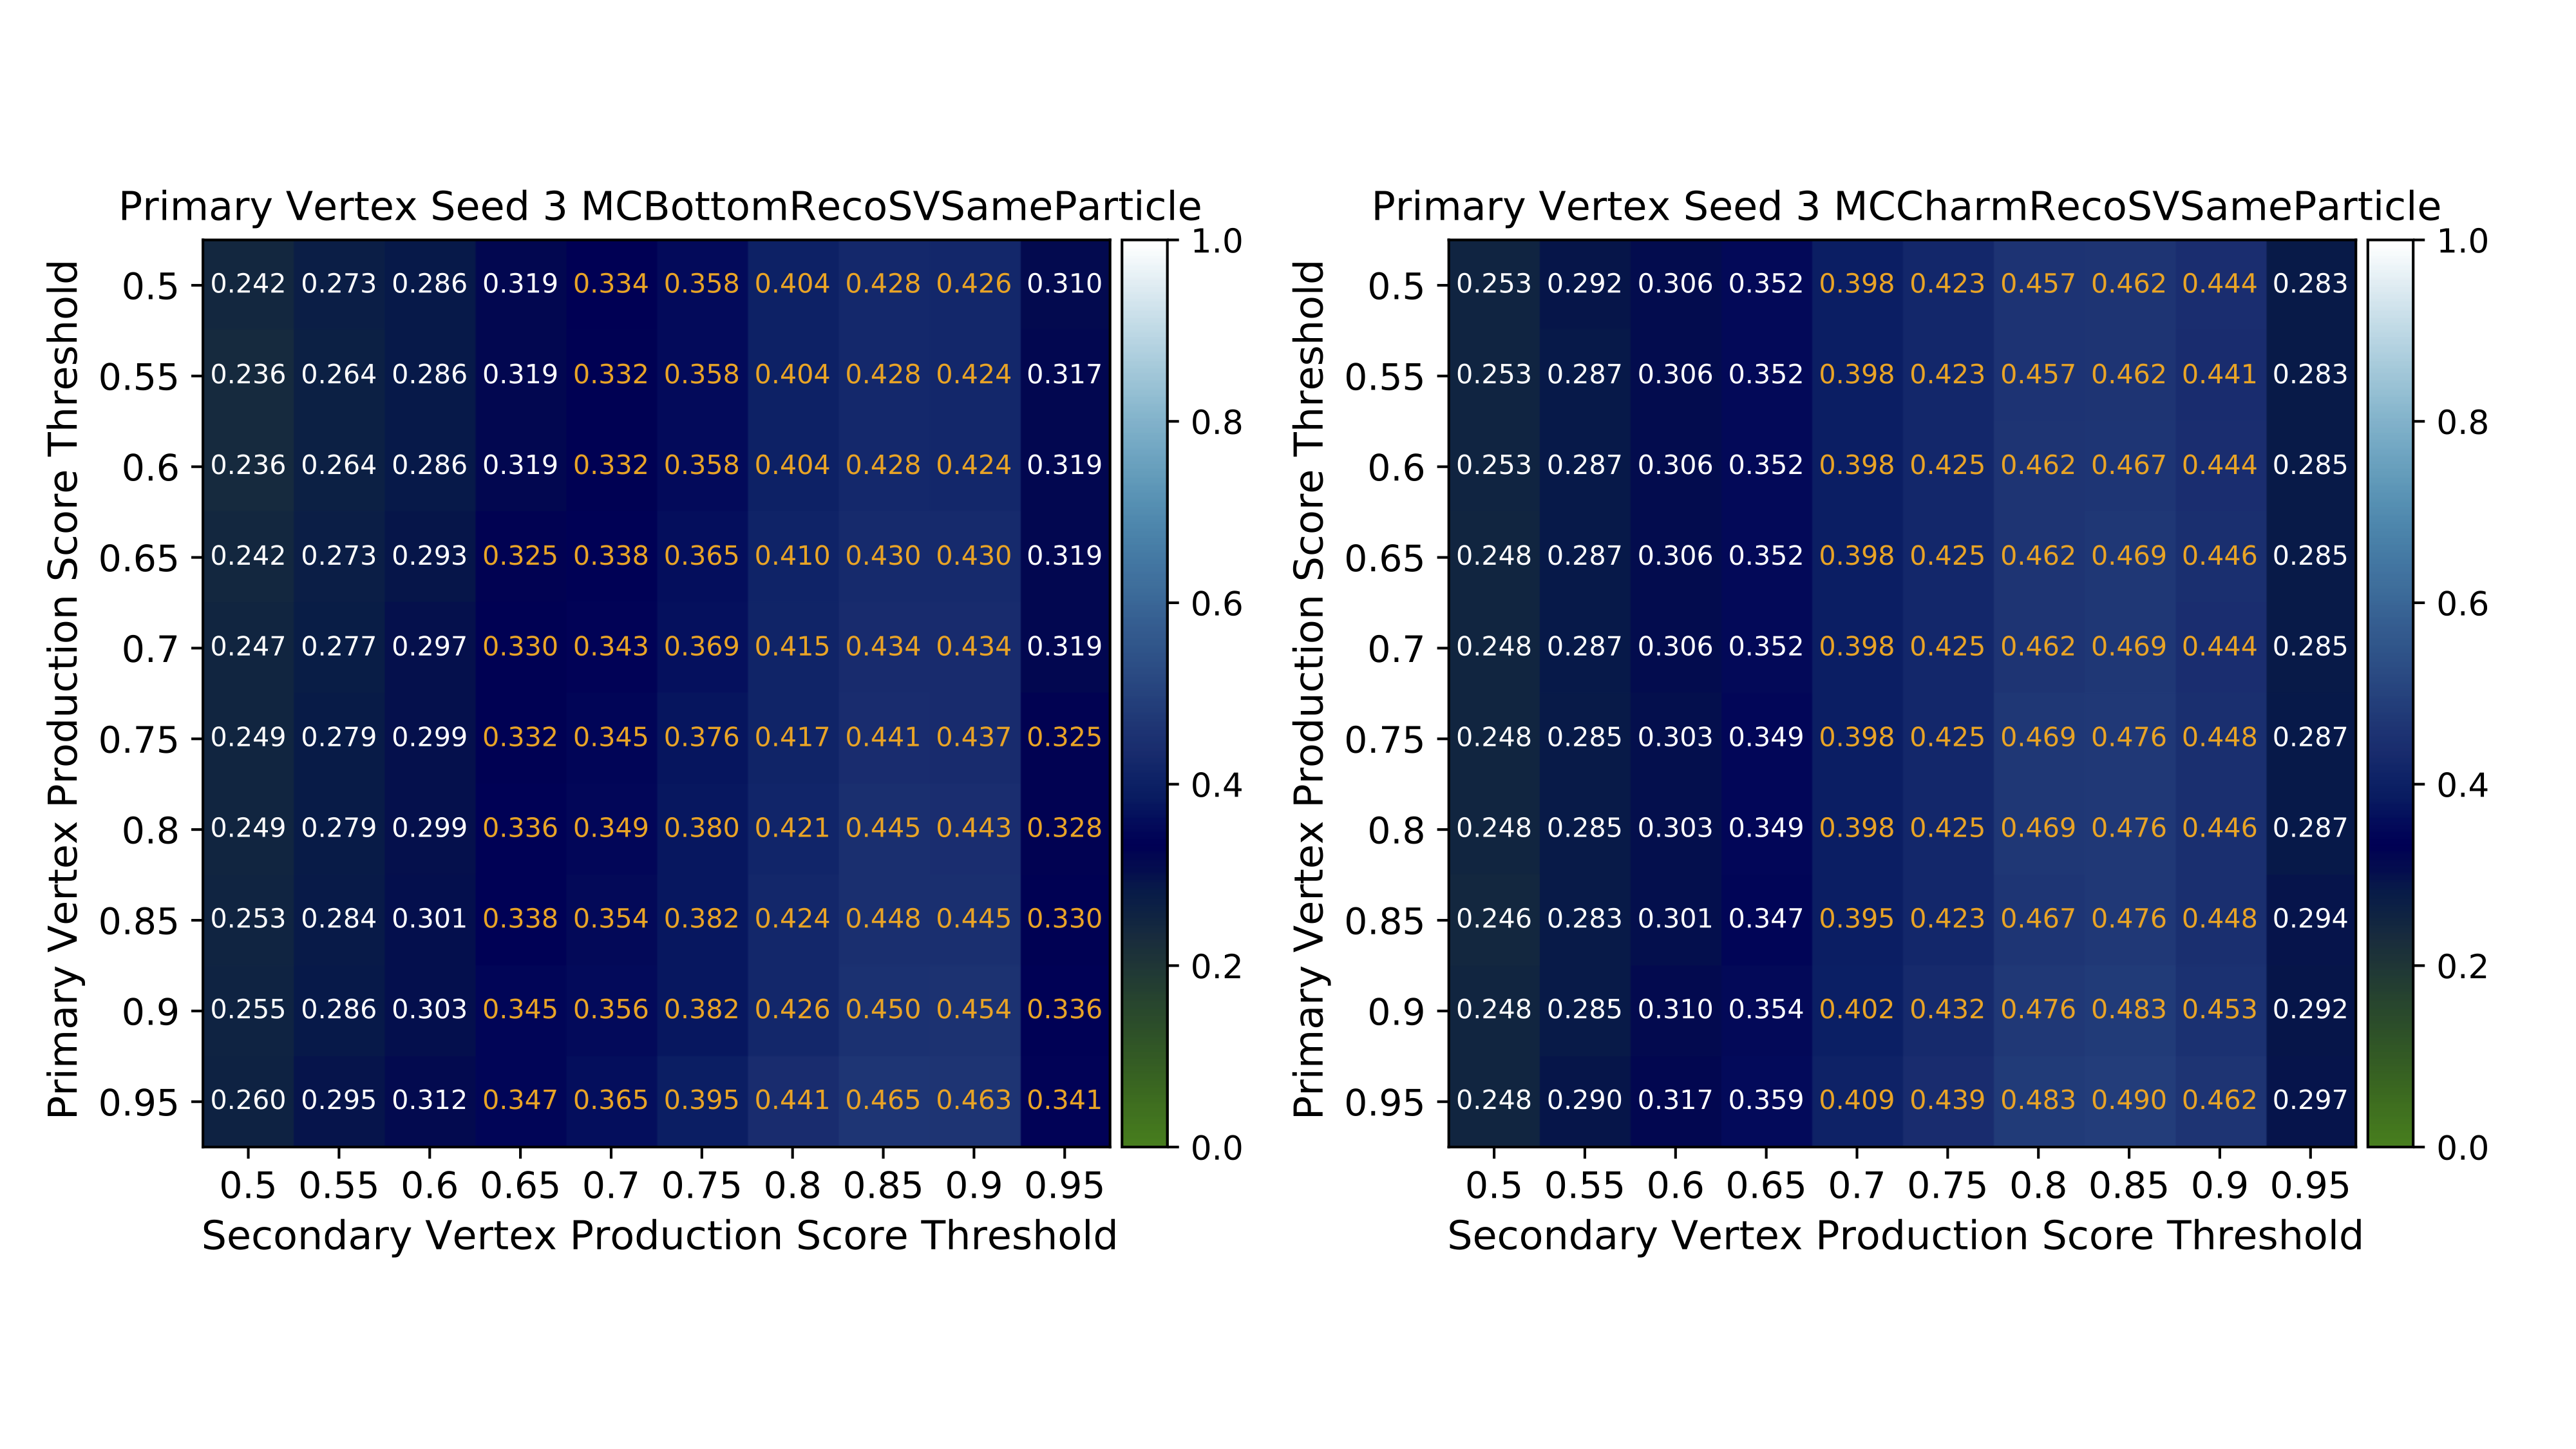
\includegraphics[trim = 0 140 0 140, width=0.95\textwidth, clip]{Figure/4VertexFinderwithDL/4-2-2-4TrackEfficiencySameParticle.png}
   \end{minipage} 
  \caption{閾値と崩壊点検出の性能の関係-PVのタネ3個}
  \label{4-2-2-4TrackEfficiency}
 %\end{tabular}
\end{figure}

ここで、次章の評価の為、現行の手法であるLCFIPlusの性能値より値の大きいものの数値を色付けしている。
SVの生成でのネットワークのスコアの閾値について同一の親粒子 (MCBottomRecoSVSameParticleやMCCharmRecoSVSameParticle) に関する性能を見ると、閾値が大きいほど値が上昇し、$0.85$付近で減少へ転じていることが分かる。
一方、MCBottomRecoSVやMCCharmRecoSVとその同一の崩壊チェイン (MCBottomRecoSVSameChainやMCCharmRecoSVSameChain) についての性能は閾値が大きいほど値が減少している。
したがって、小さな閾値では一つのSVに対して様々な飛跡が結合してしまい、結果として、同一の親粒子での性能が低下していると考えられる。
ただし、同一の崩壊チェインについては常に数\%程度の差異で追従しており、本研究のネットワークが正常に動作していることが理解できる。

MCPrimaryRecoSVやMCOthersRecoSVは非常に値が小さく、MCPrimaryRecoSVはPV、SVの生成でのネットワークのスコアの閾値の両方に感度を持っていることが分かる。
これはPVの生成に対して高い閾値を設けた場合、取り逃がした真のPV由来の飛跡がSV内に混入してしまうからである。
MCOthersRecoSVについては、PVの生成に対しての閾値について大きな影響を受けていない。
このことからPVは純度が高くOthersな飛跡をほとんど含んでいないと考えられる。


%%%%%%%%%%%%%%%%%%%%%%%%%%%%%%%%%%%%%%%%%%%%%%%%%%%%%%%%%%%%%%%%%%%%%%%%%%%%%%%%%%%%%%%%%%%%%%%%%%%%%
\section{崩壊点検出の性能} \label{VFDL:SummaryofVFDL}

本章では、現行の手法であるLCFIPlusの評価項目に則って深層学習を用いた崩壊点検出の性能を調査した。
これは次章のLCFIPlusとの比較を行う為である。

最後にデータサンプル$\rm b\bar{b}-08$での全事象を用いた性能を表\ref{PerformanceofAllEvents}に示す。
ここでは、前節で最適化を行った閾値の値として以下の組みを使用した。

\begin{itemize}
 \item SVCC・SVBB・TVCC・SVBCのスコアの和 : $0.88$
 \item 崩壊点の位置 : $30.0\ {\mathrm{mm}}$
 \item PVのタネの数 : $3$
 \item PVの生成に関するスコア : $0.75$
 \item SVの生成に関するスコア : $0.80$
\end{itemize}

\begin{table}[htb]
 \centering
 \small
  \begin{tabular}{l c c c c} \hline
    真の飛跡の種類 & Primary & Bottom & Charm & Others\\ \hline
    SVと判定された飛跡の割合 &  &  &  &\\
    ...同一の崩壊チェイン & - &  &  & - \\
    ...同一の親粒子 & - &  &  & - \\\hline
  \end{tabular}
  \caption{データサンプル$\rm b\bar{b}-08$での全事象を用いた性能}
  \label{PerformanceofAllEvents}
\end{table}



























